\section{Prepogibanje lista različnih geometrijskih oblik}
\label{pogl:prepog_geom_likov}

V tem poglavju bomo v roke vzeli liste papirja različnih geometrijskih oblik (včasih pa le navaden list papirja) in raziskovali, kaj lahko z njegovim prepogibanjem dobimo. Za uvod si bomo pogledali nekaj najosnovnejših konstrukcij, ki jih lahko učitelj matematike uporabi tudi pri pouku v osnovni šoli, nato pa se bomo vrnili nazaj v malo bolj zanimive konstrukcije, kot so konstrukcija enakostraničnega trikotnika, šestkotnika in osemkotnika. Nato si bomo pogledali vse tri Hagove izreke o razmerjih, na katere specifični pregibi kvadratnega lista papirja razdelijo njegove stranice, nato pa to posplošili na iskanje metod za razdelitev daljice na poljubno število skladnih delov. Na koncu pa bomo po konstrukciji kvadratnega korena poljubnega origami števila preko več različnih postopkov končno rešili dva starogrška problema, zaradi katerih smo se sploh začeli ukvarjati s temo origamija.

\subsection{Nekaj kratkih in zanimivih konstrukcij za uvod}

\subsubsection*{Ponazoritev lastnosti geometrijskih likov z origamijem}

Johnson v~\cite{johnson1957} opisuje, kako lahko s prepogibanjem lista papirja v obliki trikotnika, štirikotnika in kroga pokažemo določene lastnosti geometrijskih likov. Opisov, ki jih spremljajo nazorne skice konstrukcij, ne dokazuje, ampak rešitev nastavi z vprašanji, na katera mora bralec sam pri sebi odgovoriti. Učitelji so povabljeni, da se pri pouku večkrat poslužujejo teh pripomočkov, saj bo to za učence zanimivo, hkrati pa zelo poučno. Pri tem naj se sami odločijo, na kakšen način bodo uporabili prepogibanje papirja -- ali kot že podana navodila iz knjige, iz katerih morajo učenci sami ugotoviti rezultat ali kot iskanje konstrukcije, ki dokaže želeno lastnost ipd. Sedaj bomo našteli bistvene konstrukcije, ki jih navaja avtor, večinoma pa bo lažji premislek, zakaj delujejo, prepuščen bralcu.

Avtor začne z osnovami -- ki jih že poznamo -- kot so pregibi skozi točko, pravokotnica na premico (skozi dano točko, ki leži na njej ali ne), simetrala daljice, simetrala kota in vzporednica premici. Z zložitvijo trikotnika v pravokotnik na način, kot kaže slika~\ref{fig:trikotnik_vsota_kotov}, pokaže, da je vsota notranjih kotov trikotnika res $180^\circ$. Iz te konstrukcije tudi sledi formula za ploščino trikotnika, saj je le-ta dvakrat večja od ploščine nastalega pravokotnika, ki ima za stranici polovico osnovnice trikotnika in polovico njegove višine. Prav tako lahko tu vidimo, da je srednjica trikotnika (pregib vrha trikotnika na sliki ~\ref{fig:trikotnik_vsota_kotov} levo) simetrala njegove višine in pol krajša od njegove osnovnice.

\begin{figure}[h]
    \centering
    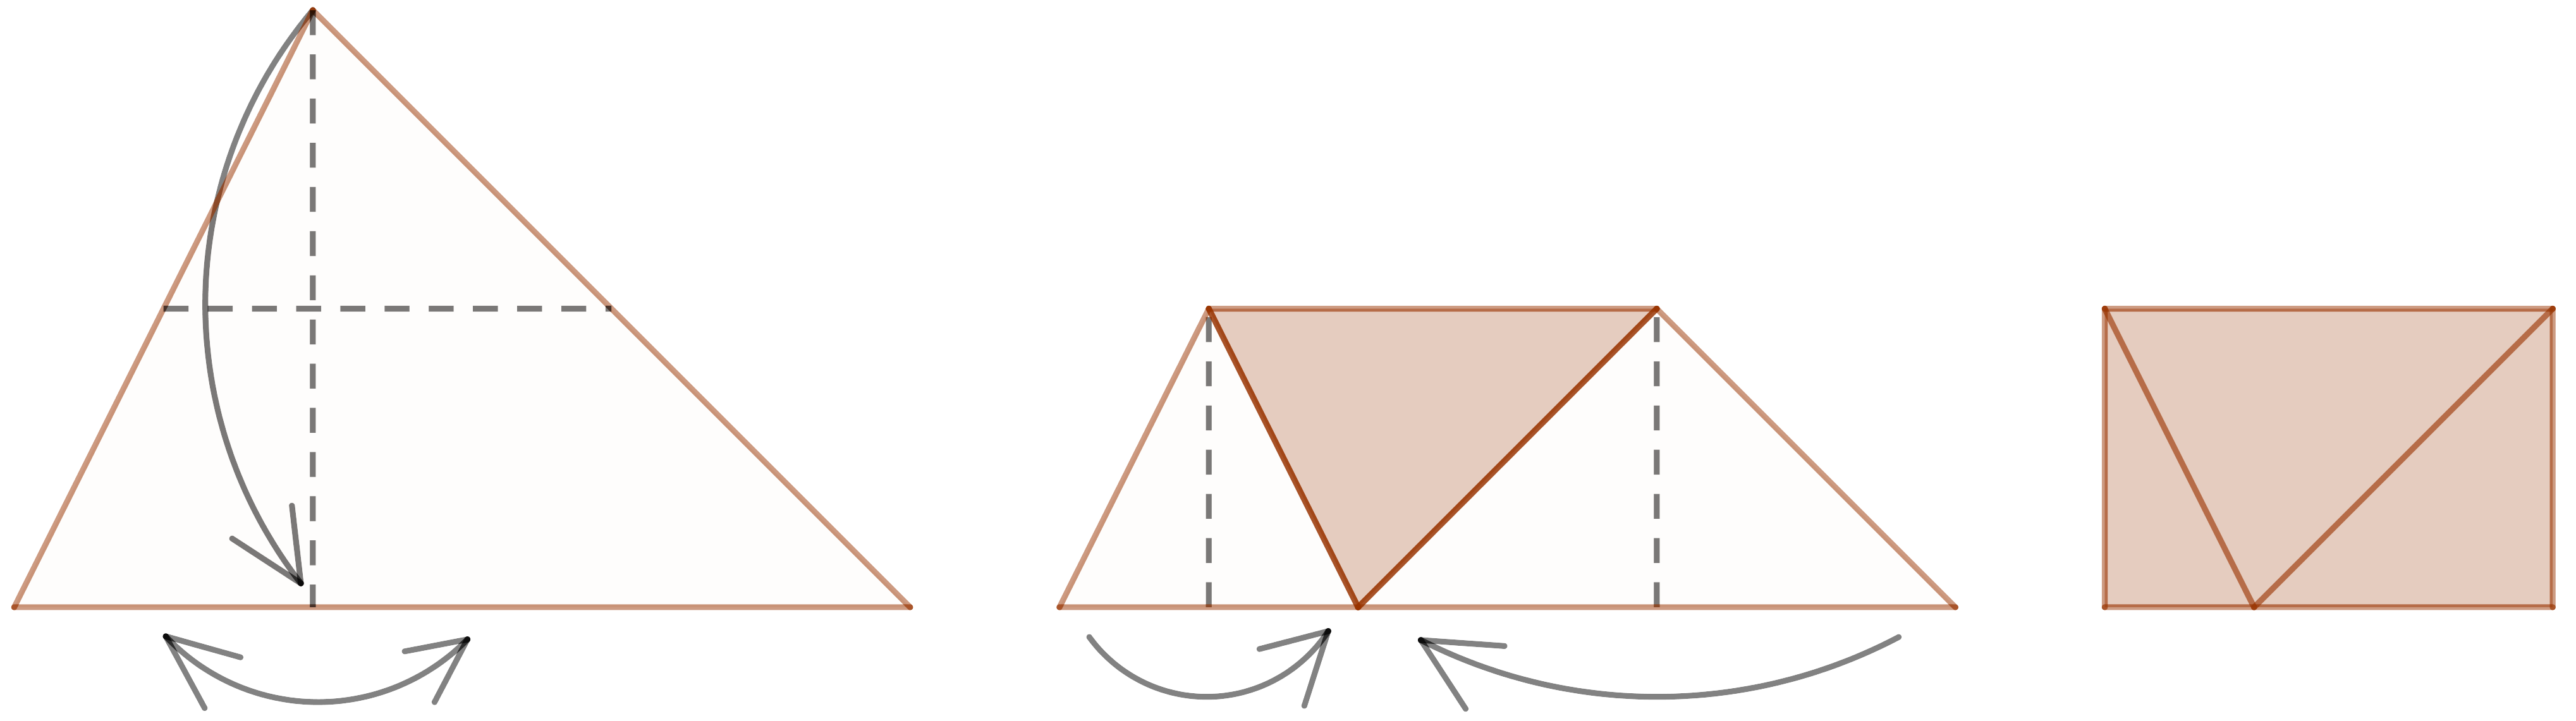
\includegraphics[width=0.8\textwidth]{images/osnovnosolski_prikazi/trikotnik_vsota_kotov.png}
    \caption[Vsota notranjih kotov trikotnika]{Pregib trikotnika, ki njegove notranje kote zloži skupaj v iztegnjeni kot.}
    \label{fig:trikotnik_vsota_kotov}
\end{figure}

Nadalje z določitvijo središča hipotenuze pravokotnega trikotnika bralca povabi, da se s prepogibi prepriča, da nastala točka osnovni trikotnik razdeli na dva enakokraka trikotnika (slika~\ref{fig:trikotnik_vec_lastnosti} levo). Prav tako se lahko prepriča, da se višine trikotnika, njegove težiščnice, simetrale stranic ter simetrale kotov sekajo v isti točki (seveda vsaka skupina daljic zase; na sliki~\ref{fig:trikotnik_vec_lastnosti} so prikazani vsi primeri razen za simetralo kotov).

\begin{figure}[h]
    \centering
    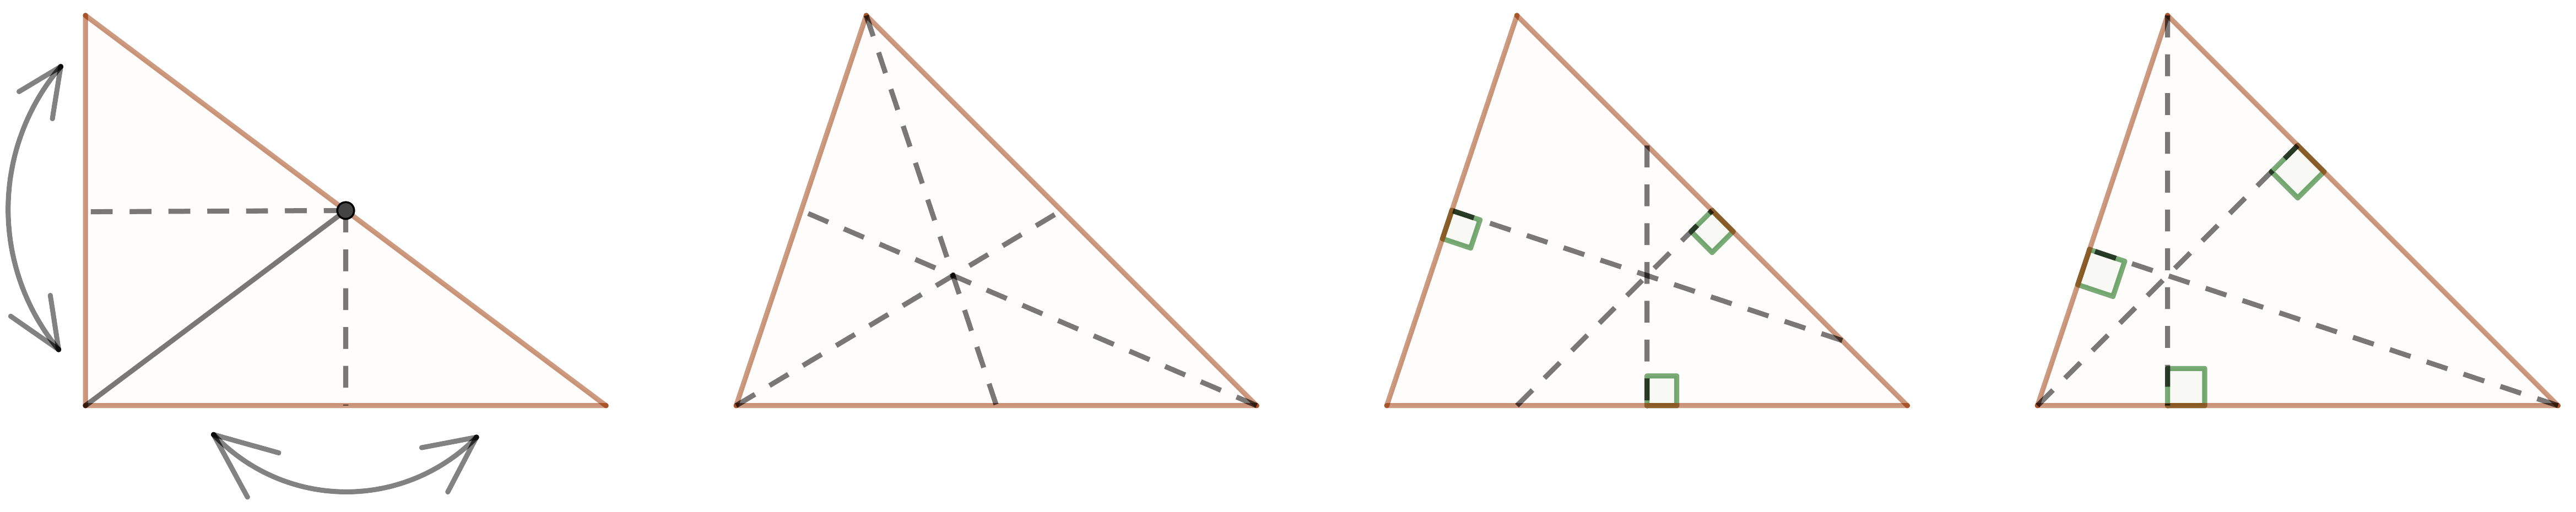
\includegraphics[width=0.95\textwidth]{images/osnovnosolski_prikazi/vec_lastnosti1.png}
    \caption[Pregibi kot dokaz lastnosti trikotnika]{Prikaz še nekaj lastnosti trikotnika.}
    \label{fig:trikotnik_vec_lastnosti}
\end{figure}

Če odložimo trikotnik in v roke vzamemo paralelogram, preko prepogib njegovih sosednjih stranic druge na drugo vidimo, da njegove diagonale v splošnem ne razpolavljajo notranjih kotov (slika~\ref{fig:par_krog_vec_lastnosti} levo). Slednje velja le za romb, za katerega poleg tega lahko še takoj s pregibom po diagonalah pokažemo, da sta pravokotni druga na drugo.

Nato se avtor posveti krogu. Vsak prepogib, ki prekrije njegove robove, ga očitno razdeli na pol in je njegov premer. Dva taka, a različna prepogiba določata središče kroga. Dobi se ga tudi tako, da prepognemo dve različni tetivi in skozi vsako izmed njiju še njeno simetralo, ki se sekata v središčni točki (slika~\ref{fig:par_krog_vec_lastnosti} na sredi). Prav tako se dva različna premera in simetrala poljubne tetive sekajo v isti točki. Avtor ravnokar naštetega ne opiše tako, temveč poda navodila za konstrukcijo pregibov in bralca sprašuje, kaj nam končna konstrukcija da. Bralec šele po opravljenih prepogibih vidi, da gre za običajne evklidske konstrukcije. Razdelek se konča še s ponazoritvijo Talesovega izreka (slika~\ref{fig:par_krog_vec_lastnosti} desno) in kosntrukcijo tangente na krožnico.

\begin{figure}[h]
    \centering
    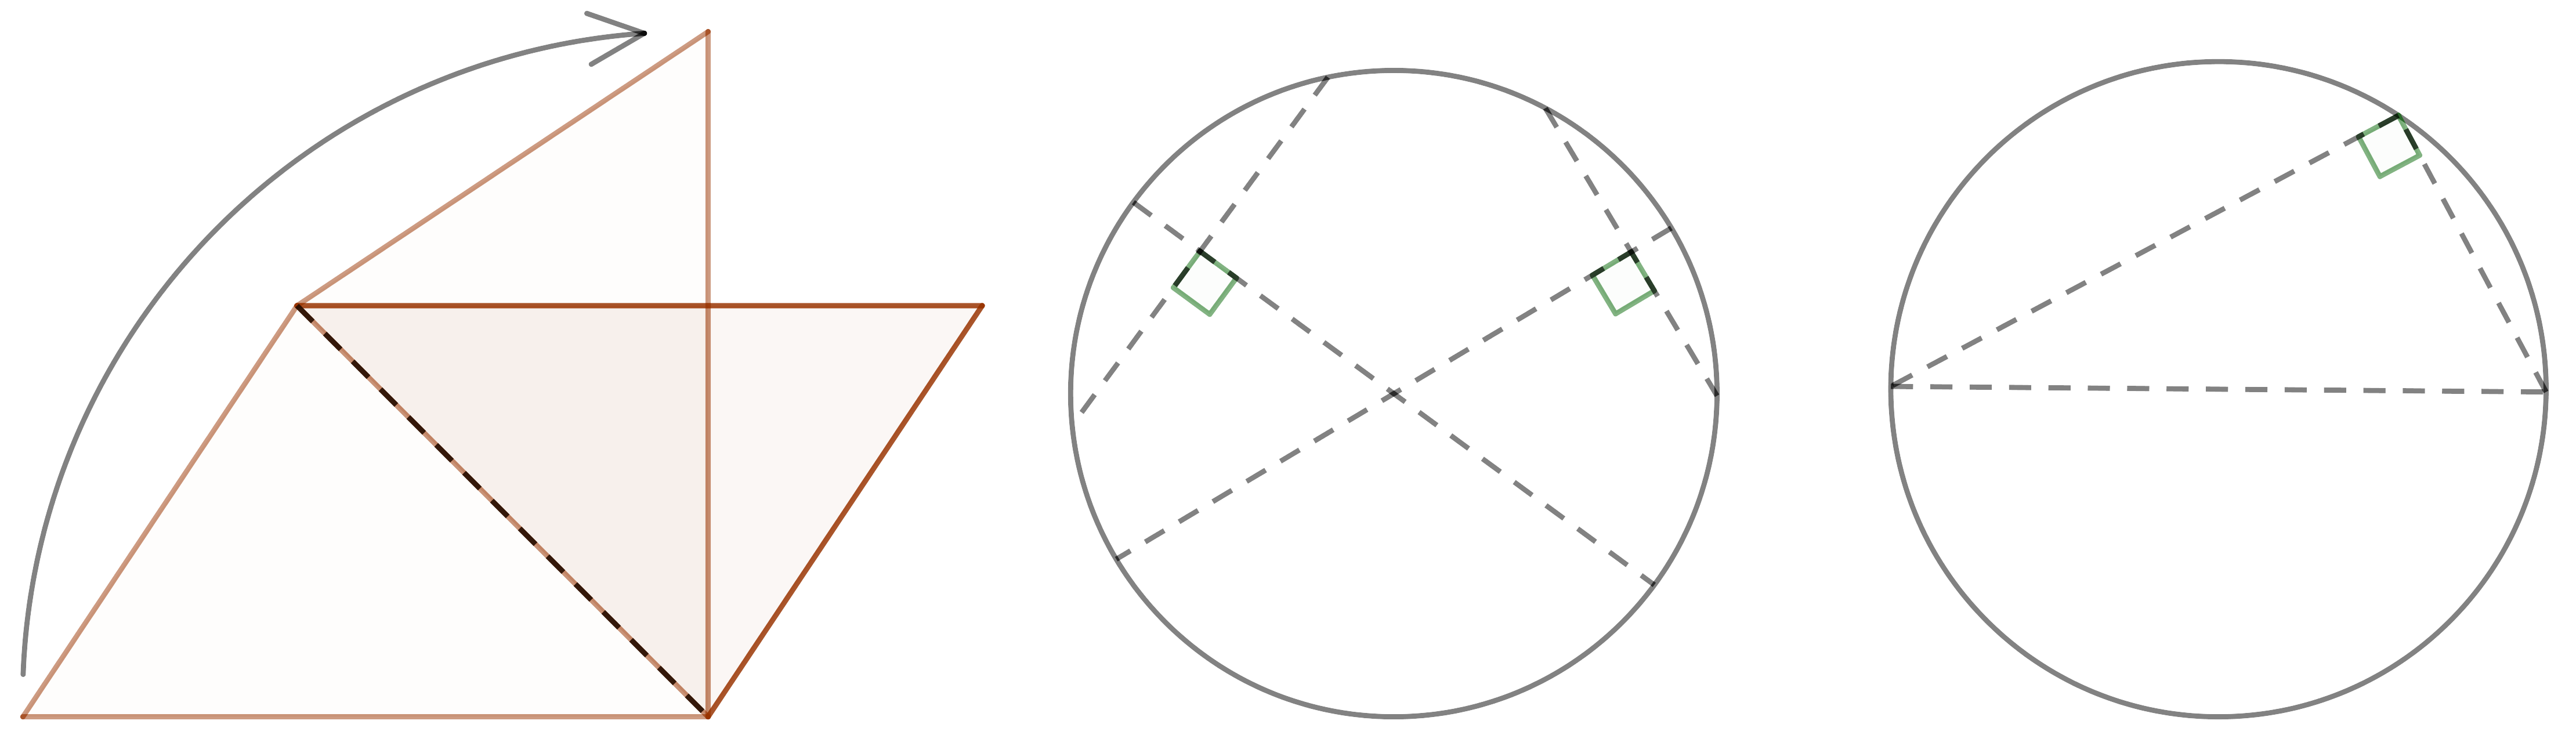
\includegraphics[width=0.9\textwidth]{images/osnovnosolski_prikazi/vec_lastnosti2.png}
    \caption[Pregibi kot dokaz lastnosti paralelograma in kroga]{Prikaz nekaj lastnosti paralelograma in kroga.}
    \label{fig:par_krog_vec_lastnosti}
\end{figure}

Nadalje lahko s prepogibanjem pravokotnika s stranicama $X$ in $X+Y$, kjer krajšo stranico prepognemo na daljšo, ponazorimo odštevanje (slika~\ref{fig:pravok_racunanje} levo). Če nato prepognemo še drugi vogal, dobimo štiri manjše pravokotnike, iz česar lahko bralec sam dokaže formulo $x^2-y^2 = (x-y)(x+y)$ (slika~\ref{fig:pravok_racunanje} desno).

\begin{figure}[h]
    \centering
    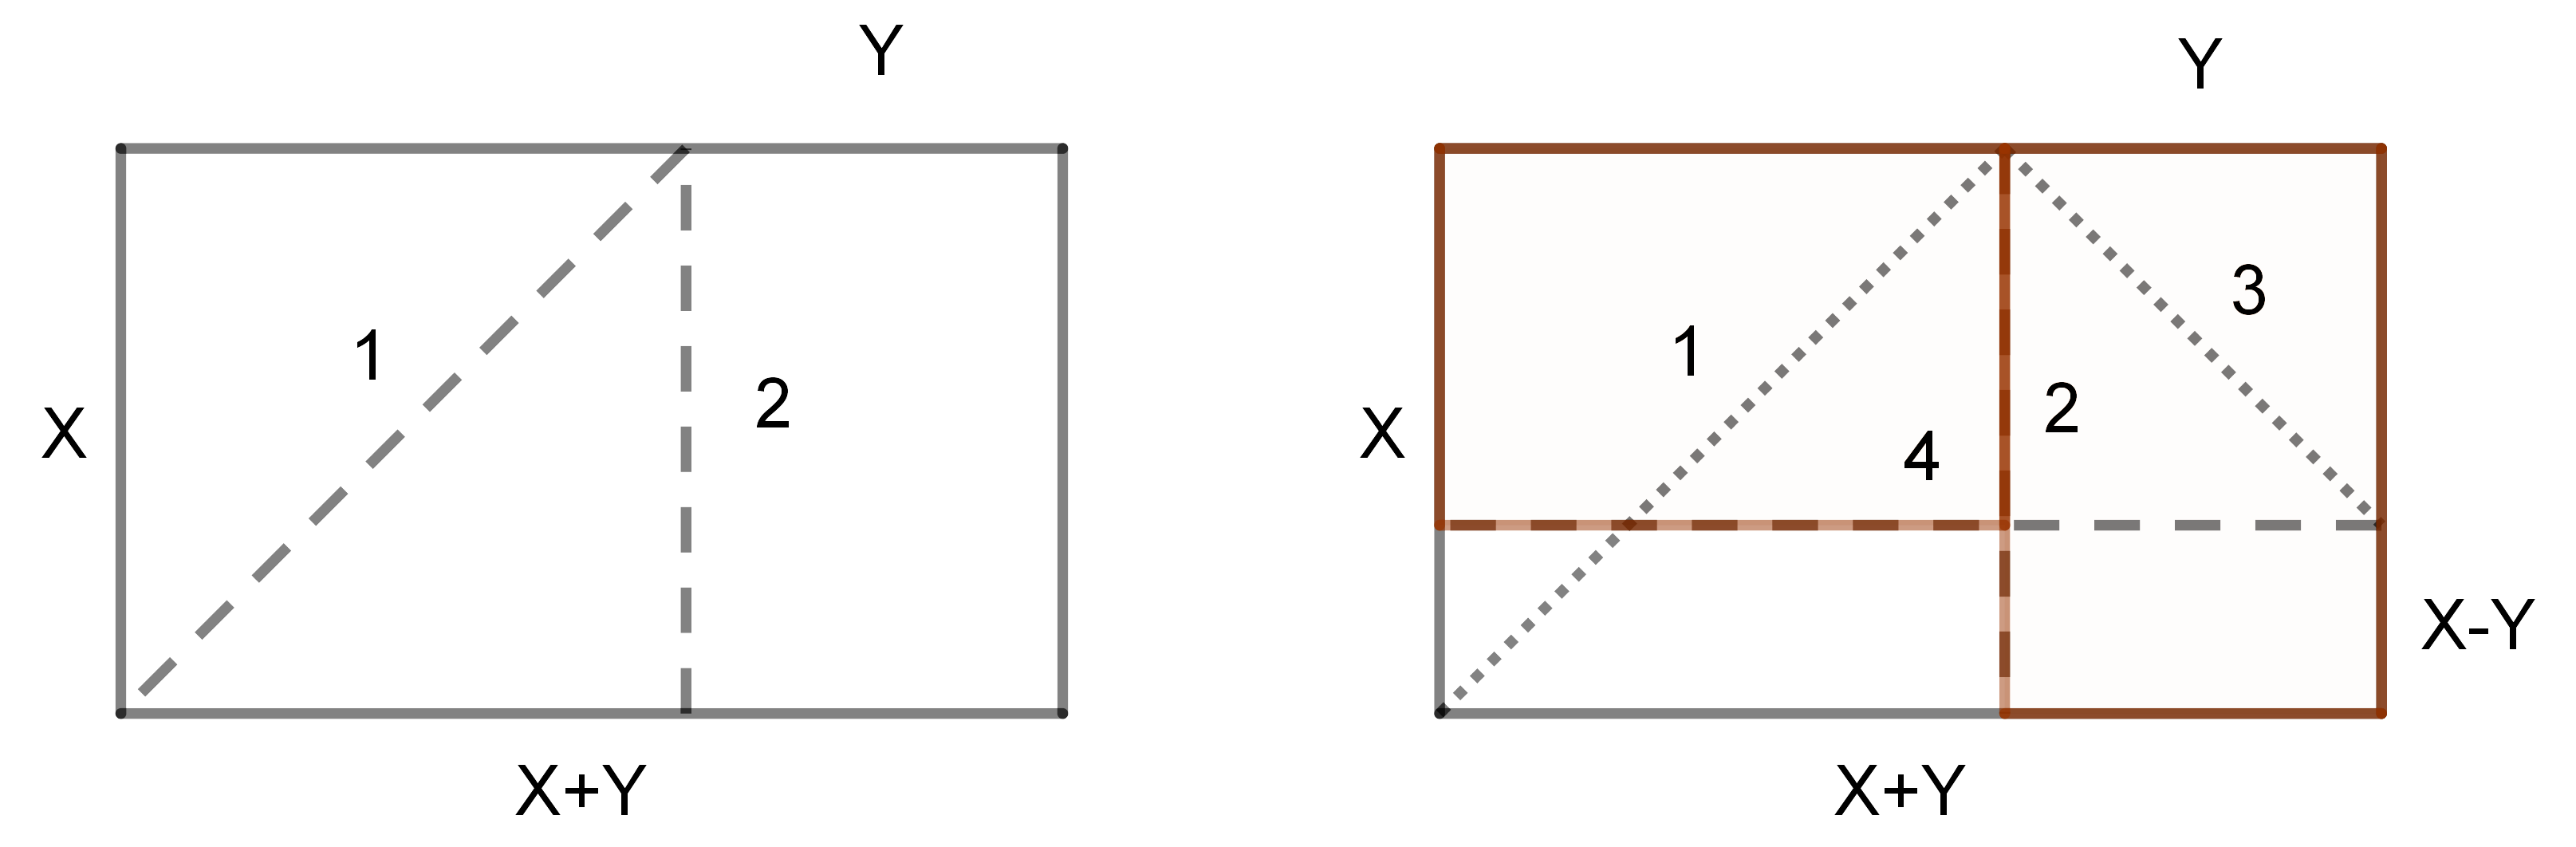
\includegraphics[width=0.8\textwidth]{images/osnovnosolski_prikazi/racunanje.png}
    \caption[Pregibi kot računanje]{Prikaz odštevanja in dokaz formule $x^2-y^2 = (x-y)(x+y)$ z označenim vrstnim redom prepogibov.}
    \label{fig:pravok_racunanje}
\end{figure}

Trije nevzporedni pregibi, ki se ne sekajo v isti točki, nam na papirju konstruirajo trikotnik. S štirimi pravokotnimi prepogibi dobimo pravokotnik, če njegovo krajšo stranico prepognemo na daljšo, pa še kvadrat (kar smo že storili pri konstrukciji v prejšnjem odstavku). V slednjem lahko z določenimi prepogibi pokažemo, da se diagonali razpolavljata in sta pravokotni druga na drugo, in če oglišča prepognemo v presečišče diagonal, dobimo nov kvadrat s polovično ploščino originalnega.

Konstrukcije poljubnega trikotnika, pravokotnika in kvadrata so zelo enostavne. Malo več premisleka pa je potrebnega za konstrukcije pravilnih $n$-kotnikov. Johnson se v nadaljevanju knjige posveti še konstrukciji $n$-kotnikov preko večkratnega zvijanja traku, simetriji, konstrukciji tangent na stožnico (kar bomo obravnavali v poglavju~\ref{pogl:stoznice}), tridimenzionalnim konstrukcijam (npr.\ kocke) in še

\subsubsection*{Konstrukcija enakostraničnega trikotnika, šestkotnika in osemkotnika}

\textcolor{red}{dej samo teve in potem za kej več referiraj poglavje o n-kotnikih}

Kvadratni list papirja po višini prepognemo na pol in nanj položimo spodnje desno oglišče $A$ kvadrata, da pregib poteka skozi spodnje levo oglišče $B$ (slika~\ref{fig:trik_enak_basic}). Sliko oglišča $A$ označimo s točko $P$. Ker je po konstrukciji $|AB| = |PB|$ in je vertikalen prepogib simetrala spodnje stranice kvadrata, je trikotnik $\triangle ABP$ enakostraničen.

\begin{figure}[h]
    \centering
    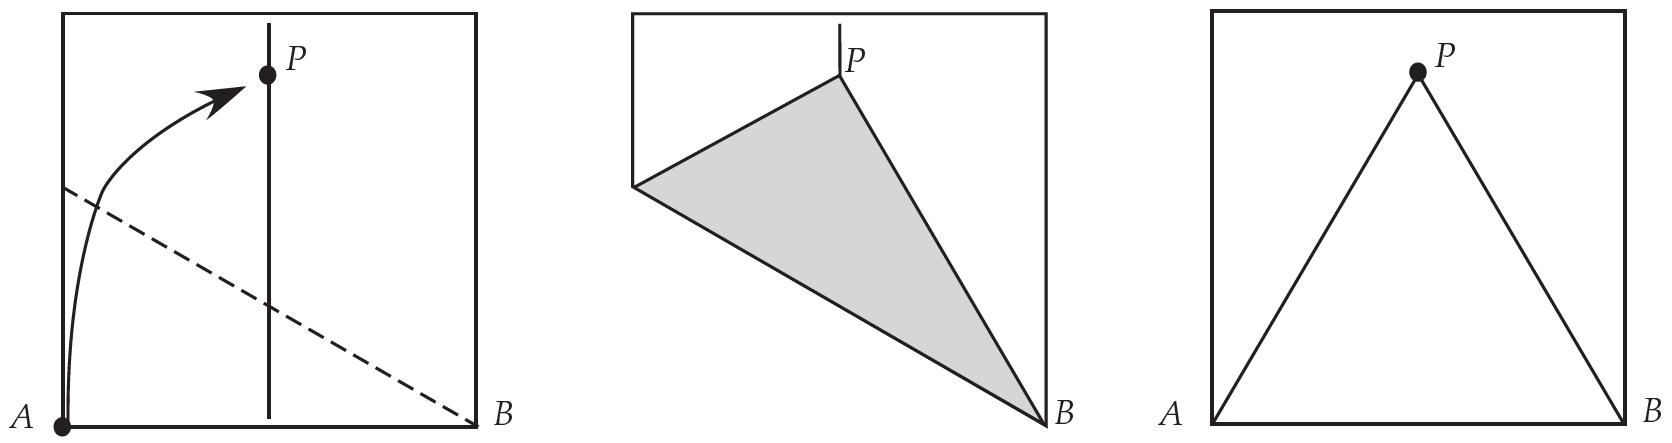
\includegraphics[width=0.9\textwidth]{images/n-kotniki/trik_enak_basic.png}
    \caption[Konstrukcija enakostraničnega trikotnika (način $1$)]{Konstrukcija enakostraničnega trikotnika. Vzeto in predelano iz~\cite[str. 9]{hull2013}.}
    \label{fig:trik_enak_basic}
\end{figure}

Sedaj, ko znamo kosntruirati enakostranične trikotnike, lahko kosntruiramo tudi pravilni šestkotnik -- kvadrat s simetralama stranic razdelimo na štiri dele, nato pa v vsakem od štirih manjših kvadratov po zgornjem postopku konstruiramo enakostranični trikotnik (oz. le eno njegovo stranico) z osnovnico na horizontalni simetrali (prve tri figure na sliki~\ref{fig:6kotnik_basic}).

\begin{figure}[h]
    \centering
    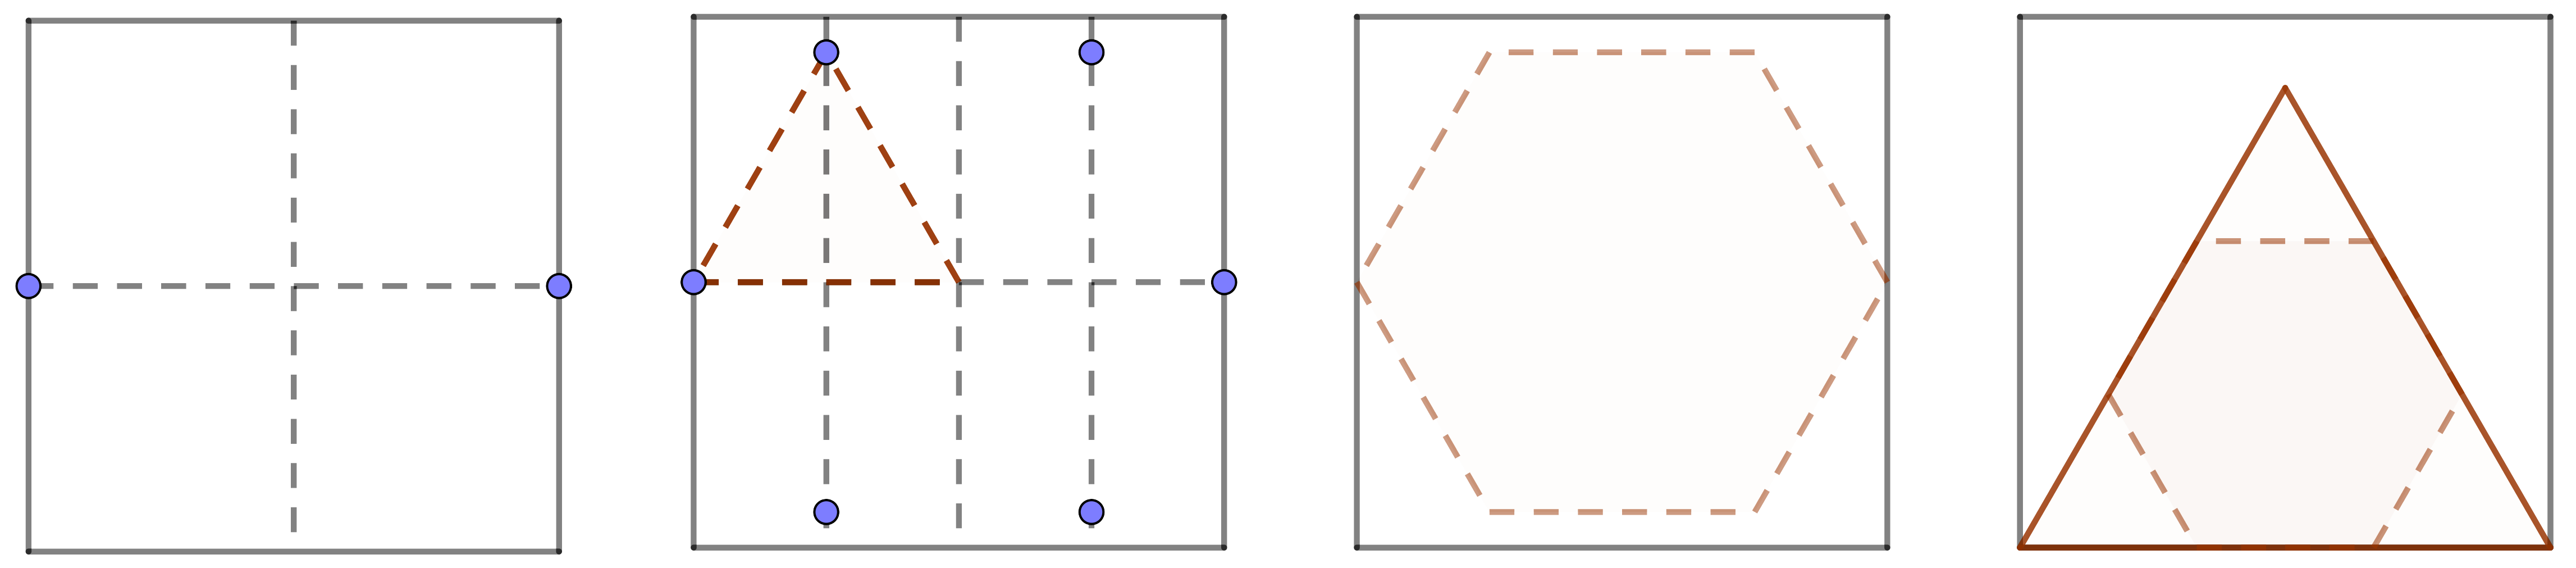
\includegraphics[width=0.95\textwidth]{images/n-kotniki/6kotnik_basic.png}
    \caption[Konstrukcija pravilnega šestkotnika (način $1$) in $2$]{Konstrukcija pravilnega šestkotnika na dva načina.}
    \label{fig:6kotnik_basic}
\end{figure}

Še lažje pravilni šestkotnik konstruiramo preko enakostraničnega trikotnika, ki mu vrhove prepognemo v središče (slika~\ref{fig:6kotnik_basic} desno). Ker središče deli višine v razmerju $2:1$, pregibi stranice razdelijo na tri skladne dele, sam trikotnik pa na tri manjše enakostranične trikotnike in šestkotnik na sredi.

V roke vzemimo nov kvadraten list papirja in konstruirajmo najprej središča njegovih stranic. S pregibi skozi sosednji središči dobimo manjši kvadrat. Sedaj razpolovimo še vsak kot, ki ga tvorita po ena stranica večjega in ena stranica manjšega kvadrata. Presečišča simetral dveh sosednjih kotov nam data še preostale štiri oglišča pravilnega osemkotnika (slika~\ref{fig:8kotnik_basic}). Bralec naj sam dokaže, da je to res.

\begin{figure}[h]
    \centering
    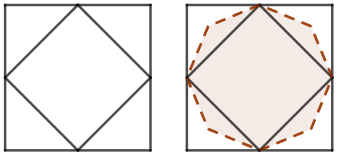
\includegraphics[width=0.5\textwidth]{images/n-kotniki/8kotnik_basic.png}
    \caption[Konstrukcija pravilnega osemkotnika]{Konstrukcija pravilnega osemkotnika.}
    \label{fig:8kotnik_basic}
\end{figure}

\textcolor{red}{S razpolavljanjem ali trisekcijo kotov ob središču kvadrata ali trikotnika -- koliko ostalih n-kotnikov lahko konstruiramo? Če je tega preveč, dej tudi to v novo poglavje ... Začneš s tem, potem pa greš na uni izrek, za koliko oglišč lahko konstruiraš z evklidskim orodjem in pol še koliko z origamijem.}

Vrnimo se nazaj na enakostranični trikotnik v danem kvadratnemu listu papirja. Ali znamo konstruirati največji tak trikotnik (in kako)? Recimo, da obstaja tak trikotnik. Najprej premislimo, da mora vsaj eno njegovo oglišče ležati v oglišču kvadrata. Če to ne drži, se trikotnik ne dotika ene stranice kvadrata -- ker ima tri stranice, kvadrat pa štiri -- recimo spodnje. Potem se z ostalimi tremi oglišči dotika preostalih treh stranic kvadrata, sicer to ne bi bil največji trikotnik -- lahko bi ga še povečali. Potisnimo sedaj trikotnik navzdol po kvadratu, dokler se najnižje oglišče na eni od pokončnih stranic kvadrata ne dotakne njegove spodnje stranice -- kar se zgodi ravno v oglišču kvadrata. Zaradi simetrije brez škode privzemimo, da je to spodnje levo oglišče.

\begin{figure}[h]
    \centering
    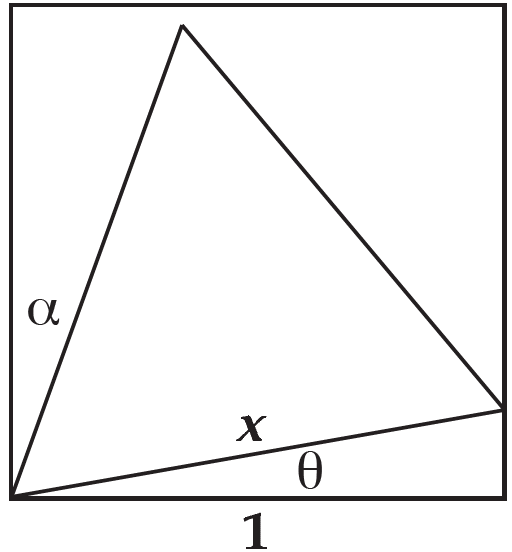
\includegraphics[width=0.25\textwidth]{images/n-kotniki/trik_enak_max1.png}
    \caption[Lega največjega enakostraničnega trikotnika znotraj kvadrata]{Lega največjega enakostraničnega trikotnika znotraj kvadrata.}
    \label{fig:trik_enak_max1}
\end{figure}

Predpostavimo, da ima kvadrat stranico dolžine $1$ in naj bo $\theta$ kot med spodnjima stranicama kvadrata in trikotnika, kot kaže slika~\ref{fig:trik_enak_max1}. Naj bo $x$ dolžina stranice trikotnika. Iščemo tak kot $\theta$, da bo ploščina trikotnika največja. Ker je notranji kot trikotnika velik $60^\circ$, je kot $\theta$ zaradi simetrije omejen z $0 \leq \theta \leq 15^\circ$. Ob upoštevanju $x = 1/ \cos \theta$ je njegova ploščina
$$ P = \frac{\sqrt{3}}{4} x^2 = \frac{\sqrt{3}}{4} \cdot \frac{1}{\cos^2 \theta}. $$
Funckijo bi lahko odvajali in preko iskanja njenega maksimuma izrazili kot, Hull pa v~\cite[str.\ 11]{hull2013} predlaga enostavnejšo rešitev. Ker je $\cos x$ na intervalu $[0^\circ, 15^\circ]$ oz.\ $[0, \pi/12]$ pozitivna in padajoča, je njena obratna vrednost naraščajoča, zato je tudi $1/\cos^2\theta$ naraščajoča funkcija. Ploščina $P(\theta)$ torej narašča in maksimum doseže pri $\theta = 15^\circ$.

Trikotnik je simetričen glede na diagonalo kvadrata. Na sliki~\ref{fig:trik_enak_max2} (levo) je prikazana konstrukcija kota $15^\circ$ -- spodnje belo območje enakostraničen trikotnik in vsak od pregibov je simetrala kota $30^\circ$. Če opravimo taka dva pregiba na sosednjih stranicah, kot kaže slika~\ref{fig:trik_enak_max2} na sredi, tako dobimo iskani največji enakostranični trikotnik v danem kvadratu.

\begin{figure}[h]
    \centering
    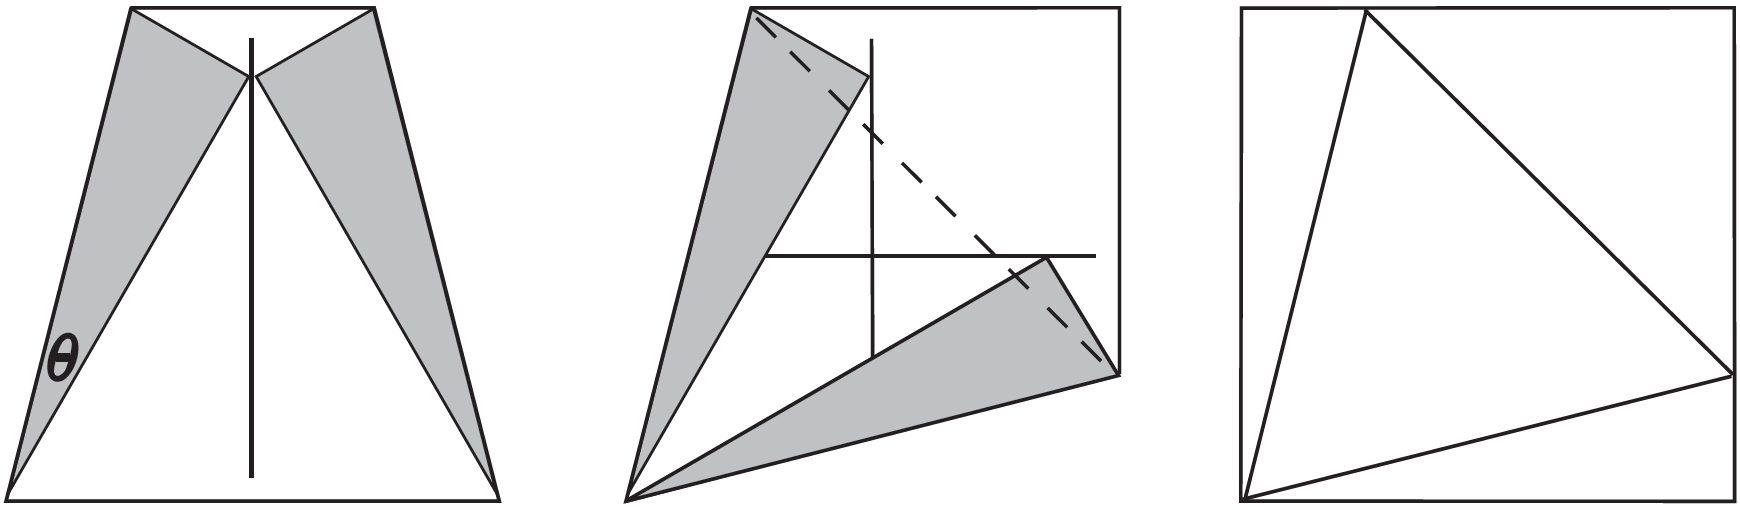
\includegraphics[width=0.9\textwidth]{images/n-kotniki/trik_enak_max2.png}
    \caption[Konstrukcija največjega enakostraničnega trikotnika znotraj kvadrata]{Konstrukcija največjega enakostraničnega trikotnika znotraj kvadrata.}
    \label{fig:trik_enak_max2}
\end{figure}

\subsection{Hagovi izreki za prepogibanje kvadrata}

S prepogibanjem kvadratnega lista papirja se je veliko ukvarjal Kazuo Haga, sicer japonski profesor biologije. V svojem delu \emph{Origamics: Mathematical Explorations Through Paper Folding}~\cite{haga2008} je tako med drugim formuliral tri izreke, ki jih poznamo pod imenom \emph{Hagovi izreki}. Pri vsakem od njih gre za konstrukcijo specifičnega pregiba, ki povzroči delitev stranic kvadrata v različnih razmerjih. Vsak izrek posebej bomo najprej formulirali, si slikovno ogledali konstrukcijo in ga dokazali, nato pa si pogledali še nekaj dodatnih lastnosti, ki sledijo iz njega.

Da si olajšamo računanje, predpostavimo, da ima kvadrat, ki predstavlja naš list papirja, stranico dolžine $1$. Njegova oglišča označimo s črkami $A, B, C$ in $D$, začenši v zgornjem desnem oglišču in sledečimi v pozitivni smeri, torej nasprotni smeri urinega kazalca.

\textcolor{red}{Konstrukcija poljubnega $a/b \in \Q$~\cite[str.\ 20--21]{lang2013}}

\textcolor{red}{Hull2013, activity 11 (str. 103--)}

\subsubsection{Prvi Hagov izrek}

\begin{izrek}[Prvi Hagov izrek]
    Zgornjo stranico $AD$ kvadrata $ABCD$ razpolovimo v točki $E$ in s pregibom nanjo položimo oglišče $C$. S tem na levi in desni stranici kvadrata dobimo tri točke, ki jih označimo z $F, G$ in $H$ (slika~\ref{fig:hagov_izrek1}). Za te točke velja:
    \begin{itemize}
        \item točka $F$ deli desno stranico v razmeru $3:5$,
        \item točka $H$ deli levo stranico v razmerju $2:1$,
        \item točka $H$ deli spodnjo stranico v razmerju $1:5$,
        \item točke $G$ deli levo stranico v razmerju $7:1$.
    \end{itemize}
\end{izrek}

\begin{figure}[h]
    \centering
    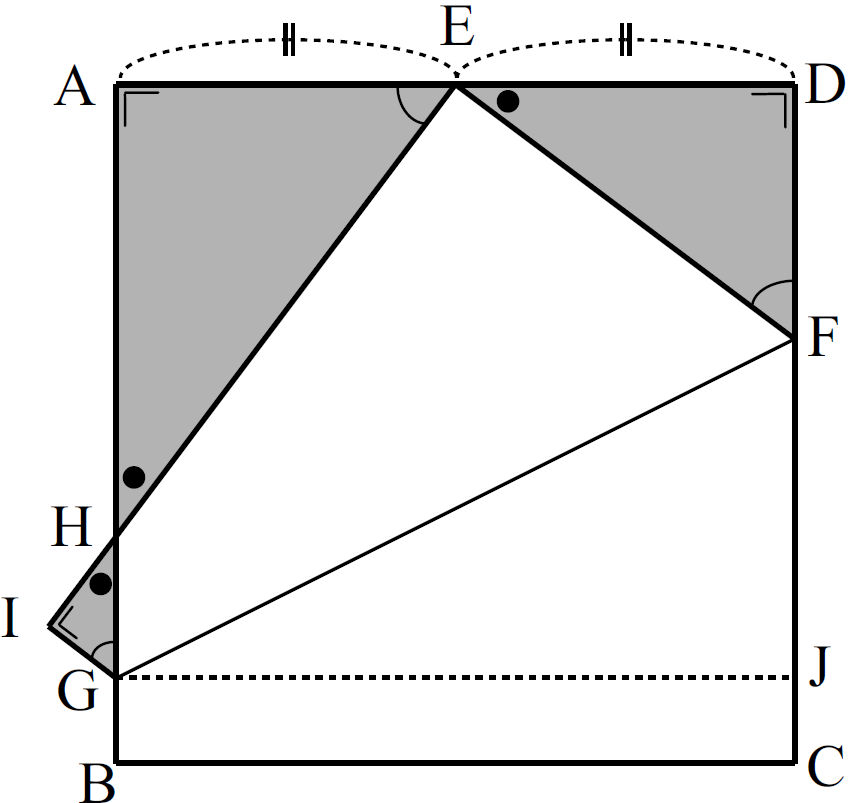
\includegraphics[width=0.4\textwidth]{images/hagovi_izreki/hagov_izrek1.png}
    \caption[Pregib iz prvega Hagovega izreka]{Konstrukcija pregiba iz prvega Hagovega izreka. Vzeto iz~\cite[str. 4]{haga2008}.}
    \label{fig:hagov_izrek1}
\end{figure}

\begin{dokaz}
    Kot kaže slika~\ref{fig:hagov_izrek1}, označimo še točki $I$ in $J$. Najprej lahko opazimo, da pregib iz izreka povzroči nastanek treh podobnih pravokotnih trikotnikov, ki so na sliki~\ref{fig:hagov_izrek1} pobarvani sivo. Za vsakega od njih lahko določimo dolžine njegovih stranic.

    Začnimo s trikotnikom $\triangle DEF$. Ker je $E$ razpolovišče stranice $AD$, je $|DE| = 1/2$. Če drugo kateto $DF$ označimo z $a$, je hipotenuza $EF$ dolga $1-a$, saj $|DF| + |EF| = |DF| + |FC| = 1$ po konstrukciji. Iz Pitagorovega izreka nato izračunamo $a = 3/8$. Torej točka $F$ res deli stranico $CD$ v razmerju $3:5$.

    Iz razmerja podobnih trikotnikov $\triangle DEF$ in $\triangle AHE$ dobimo
    $$ \frac{|AH|}{|AE|} = \frac{|DE|}{|DF|}, \; \text{ torej } \; |AH| = \frac{|AE|\cdot|DE|}{|DF|} = \frac{1/2 \cdot 1/2}{3/8} = \frac{2}{3}.$$
    Točka $H$ res deli stranico $AB$ v razmerju $2:1$. Drugače povedano -- s prvim Hagovim izrekom znamo poljubno daljico razdeliti na tri skladne dele.

    Sedaj lahko izračunamo dolžino hipotenuze $EH$ trikotnika $\triangle AHE$. Iz Pitagorovega izreka sledi $|EH| = 5/6$ (in posledično iz $|EI| = 1$ še $|HI| = 1/6$), torej točka $H$ res deli spodnjo stranico v razmerju $1:5$.

    Za izračun dolžine daljice $BG$, ki je po konstrukciji enaka dolžini katete $GI$, si spet pomagamo z razmerji podobnih trikotnikov; tokrat vzamemo trikotnika $\triangle IHG$ in $\triangle AHE$. Iz razmerja
    $$ \frac{|GI|}{|HI|} = \frac{|AE|}{|AH|} \; \text{ sledi } \; |BG| = |GI| = \frac{|AE|\cdot|HI|}{|AH|} = \frac{1/2 \cdot 1/6}{2/3} = \frac{1}{8},$$
    torej točka $G$ res deli stanico $AB$ v razmerju $7:1$.
\end{dokaz}

Za vajo lahko izračunamo še preostale dolžine daljic:
\begin{align*}
    |GH| &= |AB| - |AH| - |BG| = 1 - \frac{2}{3} - \frac{1}{8} = \frac{5}{24},\\
    |CJ| &= |BG| = \frac{1}{8},\\
    |FJ| &= |CD| - |DF| - |CJ| = 1 - \frac{3}{8} - \frac{1}{8} = \frac{1}{2},\\
    |FG| &= \sqrt{|GJ|^2 + |FJ|^2} = \sqrt{1^2 + \left(\frac{1}{2}\right)^2} = \frac{\sqrt{5}}{2}.
\end{align*}

S tem so znane vse dolžine daljic, na katere pregib iz prvega Hagovega izreka razdeli stranice enotskega kvadrata. Na sliki~\ref{fig:hagov_izrek1_st} je tako povzetek naših ugotovitev.

\begin{figure}[h]
    \centering
    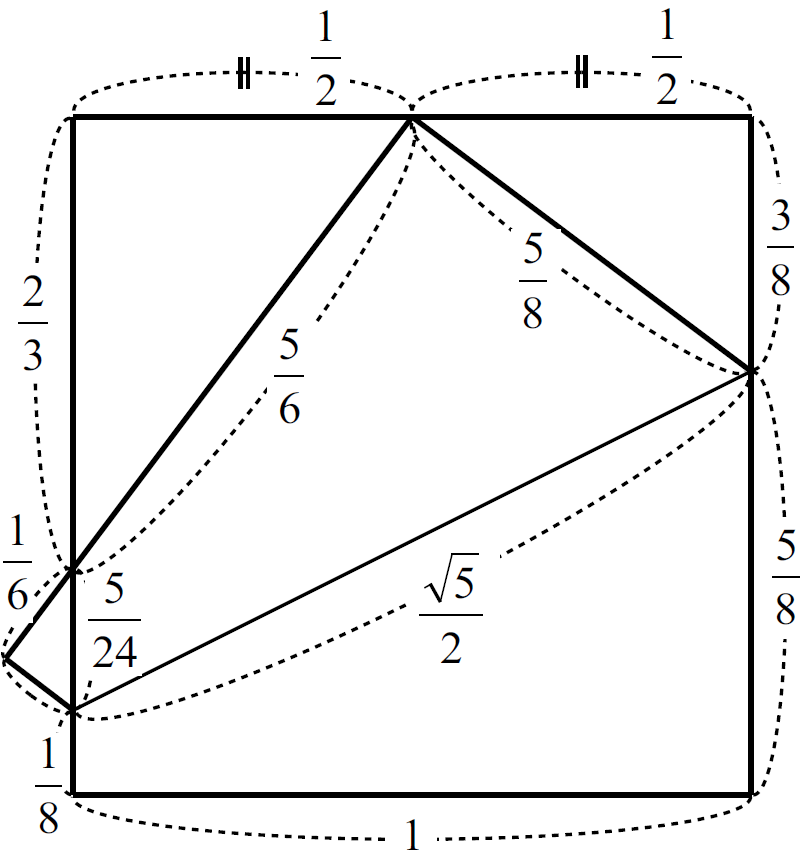
\includegraphics[width=0.4\textwidth]{images/hagovi_izreki/hagov_izrek1_stevilke.png}
    \caption[Prvi Hagov izrek v številkah]{Dolžine daljic po prvem Hagovem izreku. Vzeto iz~\cite[str. 7]{haga2008}.}
    \label{fig:hagov_izrek1_st}
\end{figure}

Izrek lahko tudi posplošimo, če za točko $E$ ne vzamemo razpolovišča, temveč poljubno točko na daljici $AD$. Naj bo $x = |ED|$. Nastale točke označimo kot prej, dolžine nastalih daljic pa z $y_1$ do $y_6$, kot kaže slika~\ref{fig:hagov_izrek1_splosen}.

\begin{figure}[h]
    \centering
    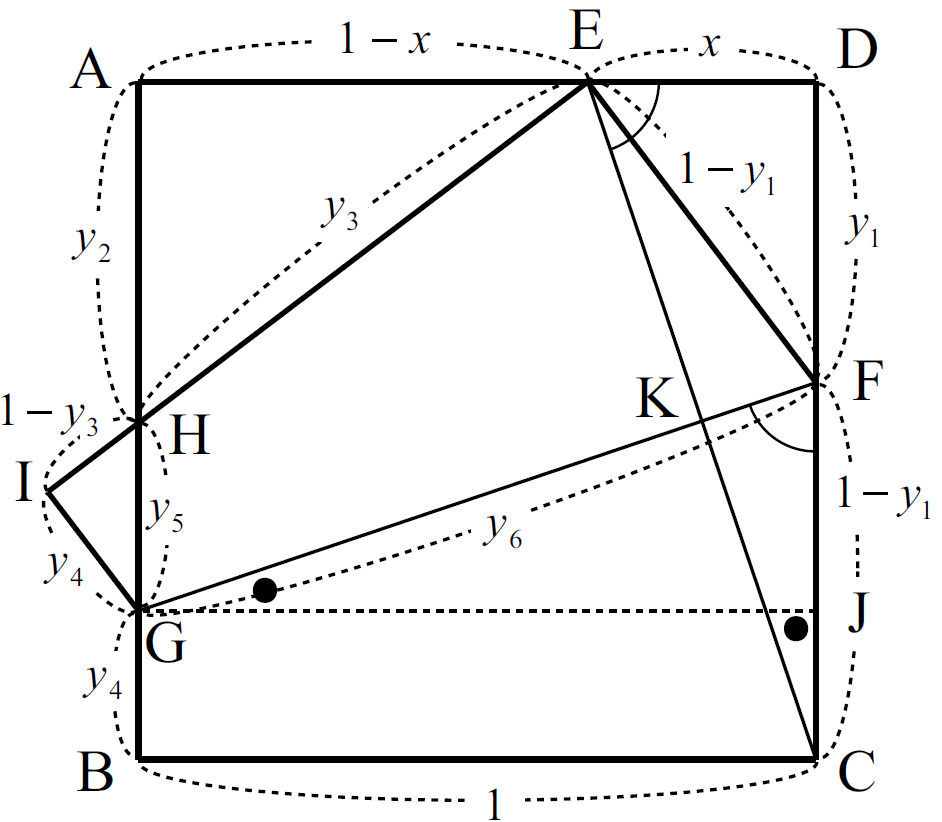
\includegraphics[width=0.5\textwidth]{images/hagovi_izreki/hagov_izrek1_splosen.png}
    \caption[Prvi Hagov izrek v splošnem]{Oznake dolžin iz prvega Hagovega izreka v splošnem. Vzeto iz~\cite[str. 9]{haga2008}.}
    \label{fig:hagov_izrek1_splosen}
\end{figure}

Za vsak $i \in \{1,2,3,4,5,6\}$ poiščimo sedaj vrednost $y_i$ v odvisnosti od $x$. Kot prej najprej opazimo, da imamo zopet tri podobne pravokotne trikotnike. Iz Pitagorovega izreka za pravokotni trikotnik $\triangle EDF$ sledi
$$y_1 = (1-x^2)/2,$$
iz razmerja podobnih pravokotnih trikotnikov $\triangle EDF$ in $\triangle HAE$ pa izračunamo
$$ y_2 = \frac{x(1-x)}{y_1} = \frac{2x}{1+x} \; \text{ in } \; y_3 = \frac{(1-y_1)(1-x)}{y_1} = \frac{1+x^2}{1+x}.$$
Pregib $FG$ je po konstrukciji simetrala daljice $CE$, torej pravokotna nanjo, iz česar sledi, da sta trikotnika $\triangle CKF$ in $\triangle CDE$ podobna in kota $\angle DEC$ in $\angle KFC$ skladna. Zato sta skladna tudi trikotnika $\triangle CDE$ in $\triangle GJF$, torej $|FJ| = x$. Posledično je
$$y_4 = |CJ| = 1 - (y_1 + x) = \frac{(1-x)^2}{2} \; \text{ in } \; y_5 = 1 - y_2 - y_4 = \frac{(1-x)(1+x^2)}{2(1+x)}.$$
Na koncu še s ponovno uporabo Pitagorovega izreka izračunamo
$$ y_6 = \sqrt{|GJ|^2 + |FJ|^2} = \sqrt{1 + x^2}.$$

Splošne vrednosti dolžin $y_i$ mogoče niso najlepše, vendar pri marsikateri izbiri števila $x \in (0,1)$ dobimo lepe številke. Najbolj so zanimiva recipročna števila naravnih števil. Vemo že, da pri izbiri $x = 1/2$ lahko dobimo števila $1/3, 1/6, 1/8$, pri izbiri $x = 1/4$ in $x = 3/4$ dobimo še $2/5$ (in iz tega z razpolovitvijo $1/5$) in $1/7$. Računanje prepuščamo bralcu, se pa na tej točki lahko vprašamo, ali za vsak $n \in \N$ obstaja primeren $x$, da lahko preko neke dolžine $y_i$ ali $1-y_1$ in preko postopkov za konstrukcijo že znanih razmerij konstruiramo dolžino $1/n$. Odgovor je pritrdilen, enostaven razmislek pa sledi v razdelku~\ref{podpogl:razdelitev_hag1_spl}.

\subsubsection{Drugi Hagov izrek}

\begin{izrek}[Drugi Hagov izrek]
    Zgornjo stranico $AD$ kvadrata $ABCD$ razpolovimo v točki $E$ in opravimo pregib skozi točko $E$ ter oglišče $C$. Točka $D$ se tako preslika v točko $F$ (slika~\ref{fig:hagov_izrek2}). Če stranico $EF$ podaljšamo do leve stranice kvadrata, jo presečišče $G$ razdeli v razmerju $2:1$.
\end{izrek}

\begin{figure}[h]
    \centering
    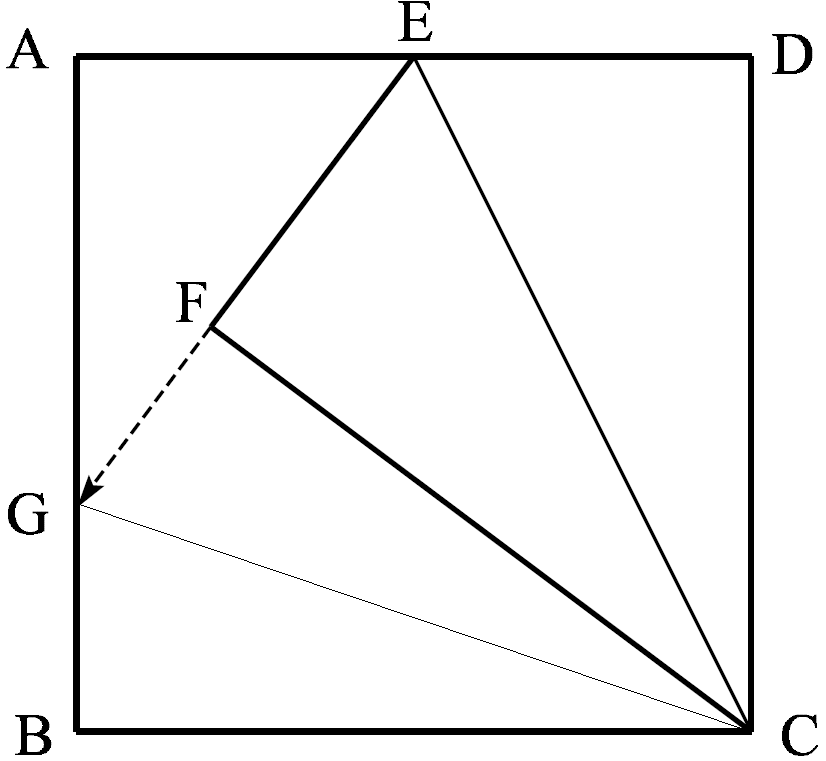
\includegraphics[width=0.4\textwidth]{images/hagovi_izreki/hagov_izrek2.png}
    \caption[Pregib iz drugega Hagovega izreka]{Konstrukcija pregiba iz drugega Hagovega izreka. Vzeto iz~\cite[str. 12]{haga2008}.}
    \label{fig:hagov_izrek2}
\end{figure}

\begin{dokaz}
    Opazimo lahko, da sta trikotnika $\triangle BCG$ in $\triangle FCG$ skladna, saj imata skladni daljšo kateto in hipotenuzo ter pravi kot nasproti hipotenuze. Označimo $x = |GB| = |GF|$. Zapišimo Pitagorov izrek za pravokotni trikotnik $\triangle AGE$:
    $$ \left(x + \frac{1}{2}\right)^2 = (1-x)^2 + \left(\frac{1}{2}\right)^2 \; \text{ in izračunamo } \; x = \frac{1}{3},$$
    torej točka $G$ res deli stranico $AB$ v razmerju $2:1$.
\end{dokaz}

S tem smo zopet dobili način razdelitve daljice na tri enake dele, a tu zanimivih razmerij še ni konec. Poglejmo si še, v kakšen razmerju nam stranice deli točka $F$ in točke, ki jih dobimo s podaljšanjem daljic $FD$ in $FC$ do leve stranice. Označimo nove točke $H, I, J, K$ in $M$, kot kaže slika~\ref{fig:hagov_izrek2_st}.

\begin{figure}[h]
    \centering
    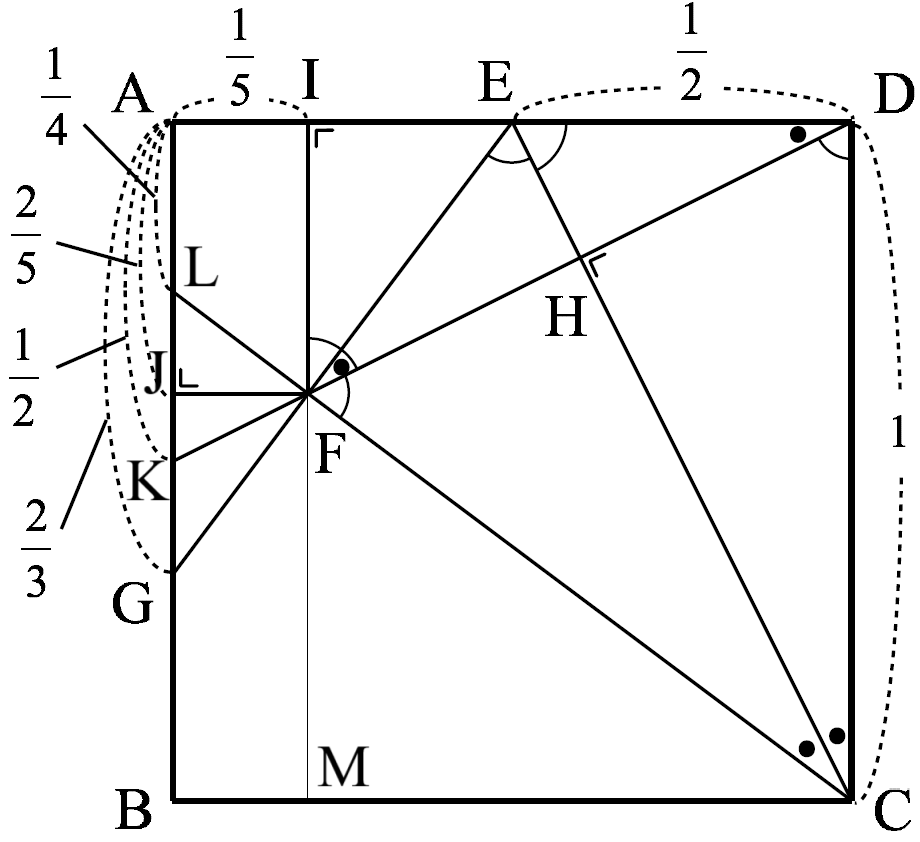
\includegraphics[width=0.45\textwidth]{images/hagovi_izreki/hagov_izrek2_stevilke.png}
    \caption[Drugi Hagov izrek v številkah]{Dolžine daljic po drugem Hagovem izreku. Vzeto in preurejeno iz~\cite[str. 15]{haga2008}.}
    \label{fig:hagov_izrek2_st}
\end{figure}

Po konstrukciji pregiba velja $FD \perp CE$, iz česar dobimo podobne pravokotne trikotnike $\triangle CDE$, $\triangle CFE$, $\triangle DAK$, $\triangle DHE$, $\triangle FHE$, $\triangle DIF$. Prvi trije od naštetih so celo skladni, prav tako je skladen tudi sledeči par. Le trikotnik $\triangle DIF$ nima skladnega para. Iz sledečih razmerij izračunamo
\begin{align*}
    |DH| &= \frac{|DE| \cdot |CD|}{|CE|} = \frac{1}{\sqrt{5}}, \; \text{ torej } \; |DF| = 2|FH| = \frac{2}{\sqrt{5}}, \\
    |DI| &= \frac{|DF| \cdot |CD|}{|CE|} = \frac{4}{5}, \; \text{ torej } \; |AI| = \frac{1}{5}, \\
    |FI| &= \frac{|DI| \cdot |DE|}{|CD|} = \frac{2}{5} \; \text{ in} \\
    |AK| &= |DE| = \frac{1}{2}.
\end{align*}

Iz podobnih trikotnikov $\triangle BCL$ in $\triangle MCF$ sledi še
$$ |BL| = \frac{|BC| \cdot |FM|}{|CM|} = \frac{3}{4}, \; \text{ torej } \; |AL| = |AB| - |BL| = \frac{1}{4}. $$

Torej nam drugi Hagov izrek poleg konstrukcije števil $1/3, 2/3$ poda tudi diretkno konstrukcijo števil $1/5, 2/5, 3/5$ in $4/5$.

\subsubsection{Tretji Hagov izrek}

\begin{izrek}[Tretji Hagov izrek]
    Zgornjo stranico $AD$ kvadrata $ABCD$ razpolovimo v točki $E$ in opravimo pregib, ki točko $E$ položi na desno stranico in hkrati oglišče $C$ na levo stranico (slika~\ref{fig:hagov_izrek3}). Njena slika $H$ levo stranico deli v razmerju $2:1$.
\end{izrek}

\begin{figure}[h]
    \centering
    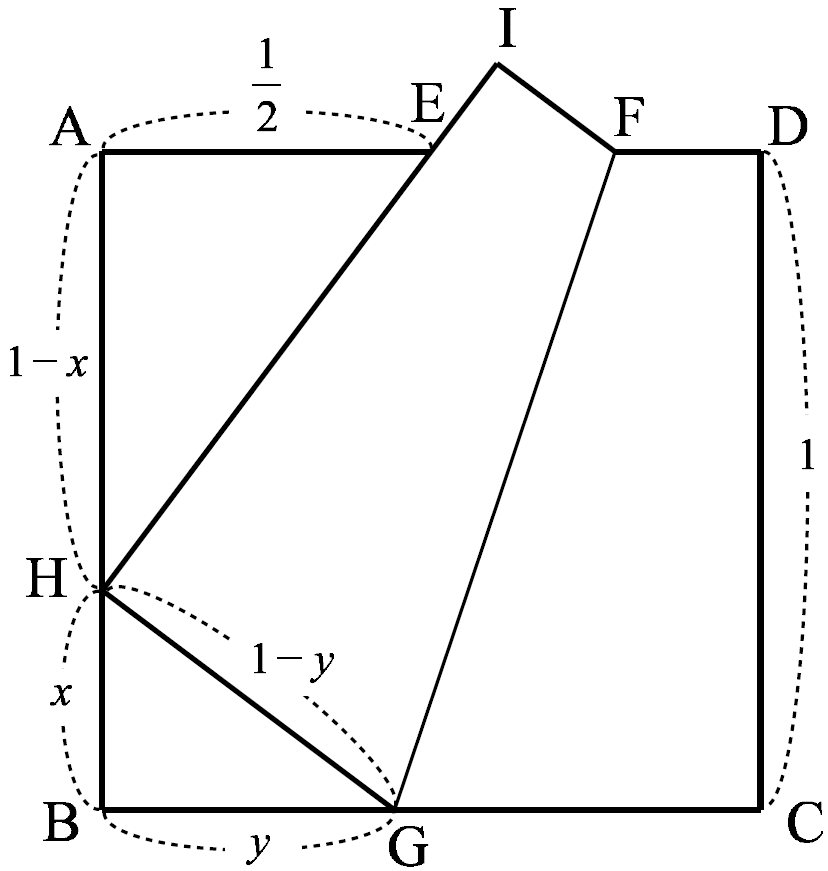
\includegraphics[width=0.4\textwidth]{images/hagovi_izreki/hagov_izrek3.png}
    \caption[Pregib iz tretjega Hagovega izreka]{Konstrukcija pregiba iz tretjega Hagovega izreka. Vzeto iz~\cite[str. 18]{haga2008}.}
    \label{fig:hagov_izrek3}
\end{figure}

\begin{dokaz}
    Označimo še točke $E, F, G,$ in $I$ ter uvedimo $x = |BH|$ in $y = |BG|$, kot kaže slika~\ref{fig:hagov_izrek3}. Zaradi prepogiba je $|GH| = |CG| = 1-y$. Iz Pitagorovega izreka za pravokotni trikotnik $\triangle BGH$ ter razmerja za podobna trikotnika $\triangle BGH$ in $\triangle AHE$ dobimo sistem enačb
    $$ x^2 + y^2 = (1-y)^2 \; \text{ in } \; \frac{1/2}{1-x} = \frac{x}{y}, $$
    iz katerih izračunamo $x = \frac{1}{3}$ in $y = \frac{4}{9}$. Torej točka $H$ res deli stranico $AB$ v razmerju $2:1$.
\end{dokaz}

Kot pri prejšnjih dveh izrekih bi lahko poračunali še preostale dolžine daljic. To za vajo prepuščamo bralcu, ki se lahko o svojih rezultatih prepriča s sliko~\ref{fig:hagov_izrek3_st}.

\begin{figure}[h]
    \centering
    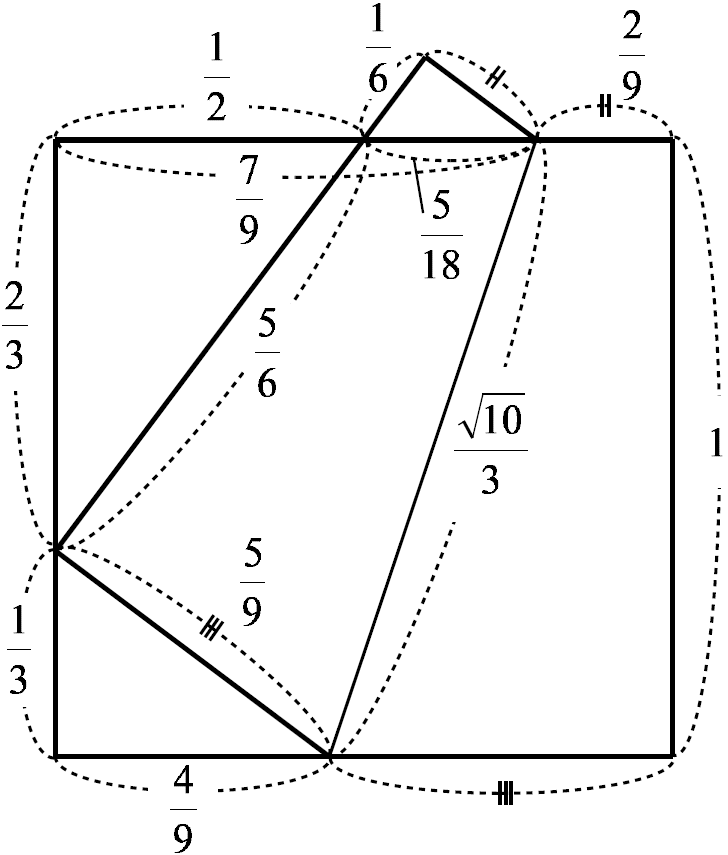
\includegraphics[width=0.4\textwidth]{images/hagovi_izreki/hagov_izrek3_stevilke.png}
    \caption[Tretji Hagov izrek v številkah]{Dolžine daljic po tretjem Hagovem izreku. Vzeto iz~\cite[str. 19]{haga2008}.}
    \label{fig:hagov_izrek3_st}
\end{figure}


\textcolor{red}{Kakšen zaključek teh treh izrekov? Skupno -- vsi trije uporabljajo središče $E$ zgornje stranice $AD$. Prvi izrek nanj položi oglišče $C$, drugi izrek naredi pregib skoznjo in oglišče $C$, tretji pa nanjo položi desno stranico tako, da $C$ leži na levi stranici. Kej skupnega, bi se dalo še kakšen drug pregib blablabla}

\textcolor{red}{Lahko omeniš še srebrne pravokotnike (npr.\ A4 list papirja, stranici sta v razmerju $1 : \sqrt{2}$ in vsakič, ko daš pravokotnik po kratki stranici na pol, dobiš spet srebrn pravokotnik; pač isti princip kot pri zlatem pravokotniku za zlati rez), pa da se da tudi na njih naredit te Hagove izreke. Katere razdelitve dobiš? Na 9, 14, 16 delov itd., poglej vir. Ampak to nej gledajo v~\cite[str.\ 21--32]{haga2008}.}



\subsection{Razdelitev daljice na $n$ enakih delov}

Stranico kvadrata želimo razdeliti na $n$ enakih delov, kjer je $n \in \N$ poljuben. Za $n = 2^t$, kjer je $t \in \N_0$, je to čisto enostavno, saj samo prepolavljamo razdalje med pregibi, dokler ne dosežemo cilja. Če je $n$ sod, vendar ni potenca $2$, torej $n = 2^t(2m + 1)$, kjer sta $t, m \in \N$, stranico najprej razdelimo na $2^t$ delov, nato pa moramo vsakega izmed njih razdeliti na $2m + 1$ (liho število) delov. Izziv tega problema je torej v razdelitvi daljice na liho število delov. Ko bomo zo zmogli, jo bomo znali razdeliti na $n$ delov za vsak $n \in \N$.

V prejšnjem razdelku so nam Hagovi izreki podali razdelitev stranice kvadrata na tri, pet, sedem in devet delov. Vendar iščemo metodo, ki nam stranico razdeli na $n$ delov za splošen lih $n \in \N$. Spomnimo se, da smo en tak postopek že spoznali -- v dokazu izreka~\ref{izr:podpolje} smo za poljuben $a \in \R$ znali konstruirati razdaljo $1/a$, kar bi lahko uporabili za razdelitev neke daljice na $a$ enakih delov -- konstruirano razdaljo $1/a$ bi $a$-krat prenesli naprej. Načinov reševanja tega problema pa se je skozi zadnja desetletja oblikovalo še veliko več; tu si bomo pogledali še \textcolor{red}{koliko?} metode.

\subsubsection*{Metoda križajočih se diagonal}

Metoda nima uradnega prevoda niti uradnega imena, jo pa tako imenuje Robert J.\ Lang v svojem članku~\cite{lang1988}. Njena konstrukcija je prikazana na sliki~\ref{fig:kriz_diag_3}. Najprej kvadrat dvakrat prepognemo na pol -- enkrat po diagonali skozi oglišči $A$ in $C$ in drugič po vertikali. Nato prepognemo po diagonali (skozi oglišče $B$) še desni pokončen pravokotnik. Presečišče obeh diagonal označimo s točko $P$ in naredimo skoznjo prepogib, ki je pravokoten na horizontalno stranico kvadrata.

\begin{figure}[h]
    \centering
    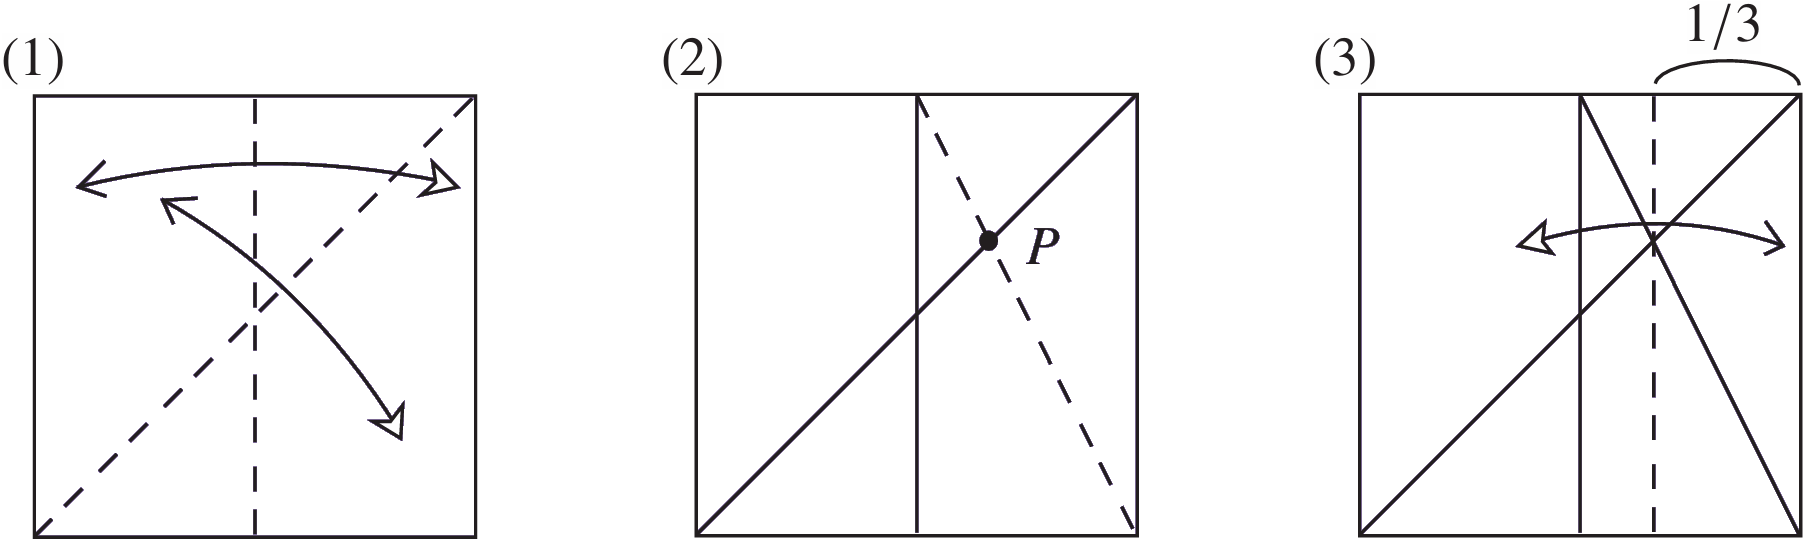
\includegraphics[width=0.9\textwidth]{images/tretjinjenje_stranice1.png}
    \caption[Razdelitev stranice na tri dele]{Konstrukcija po metodi križajoih se diagonal za $n=3$. Vzeto in preurejeno iz~\cite[str. 37]{hull2013}.}
    \label{fig:kriz_diag_3}
\end{figure}

\begin{trditev}[Metoda križajočih se diagonal za $n=3$]
    \label{trd:kriz_diag_3}
    Zadnji pregib iz zgornjega opisa konstrukcije razdeli horizontalno stranico kvadrata v razmerju $2:1$.
\end{trditev}

\begin{dokaz}
    Dokazujemo lahko na več načinov:
    \begin{enumerate}
        \item \textit{Analitičen pristop:} Kvadrat postavimo v evklidsko ravnino tako, da leži oglišče $A$ v koordinatnem izhodišču in oglišče $B$ v točki $(1, 0)$. Obe diagonali izrazimo z enačbama premic. Glavna diagonala ima enačbo $y = x$, diagonala pravokotnika pa $y = -2x + 2$. Točka $P$ je njuno presečišče in ima tako koordinati $(2/3, 2/3)$.
        \item \textit{Preko podobnih trikotnikov:} Z opisanimi prepogibi v tem kvadratu konstruiramo več trikotnikov. Njihova oglišča označimo tako, kot kaže slika~\ref{fig:kriz_diag_3_dokaz}. Iz podobnosti trikotnikov $\triangle AGP$ in $\triangle ABC$ sledi, da je trikotnik $\triangle AGP$ enakokrak. Naj bo dolžina njegovih krakov $x$. Potem je $|AG| = |GP| = x$ in $|GB| = 1 - x$. Iz podobnosti trikotnikov $\triangle EFB$ in $\triangle PGB$ sledi
        \begin{align*}
            \frac{|EF|}{|FB|} &= \frac{|PG|}{|GB|}, \\
            \frac{1}{\frac{1}{2}} &= \frac{x}{1 - x}, \\
            x &= \frac{2}{3}.
        \end{align*}
        \begin{figure}[h]
            \centering
            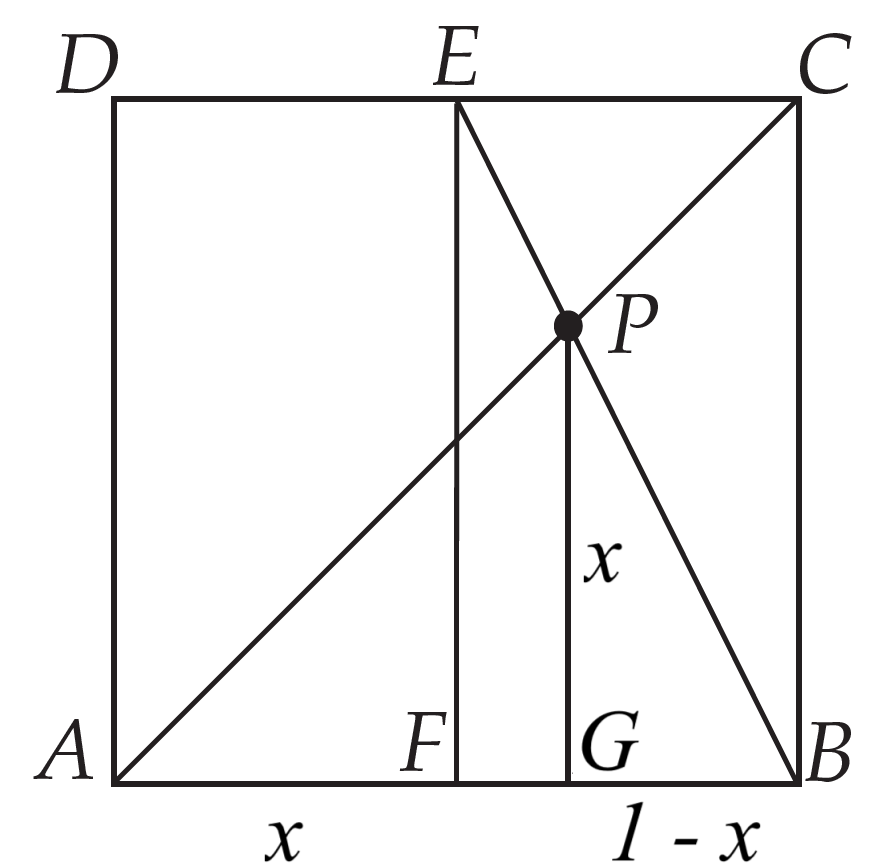
\includegraphics[width=0.3\textwidth]{images/tretjinjenje_stranice2.png}
            \caption[Dokaz metode križajočih diagonal]{Dokaz metode križajočih se diagonal za $n=3$. Vzeto in preurejeno iz~\cite[str. 38]{hull2013}.}
            \label{fig:kriz_diag_3_dokaz}
        \end{figure}
    \end{enumerate}
\end{dokaz}

Po konstrukciji pregiba, ki zgornjo stranico kvadrata razdeli v razmerju $2:1$, levi pravokotnik (s stranico $AG$) po vertikali prepognemo še na pol in tako stranico kvadrata razdelimo na tri enake dele. Preidimo sedaj iz $n = 3$ na višje število delov.

Razdelitev stranice kvadrata na štiri dele je že znana -- kvadrat v vertikalni smeri dvakrat prepognemo na pol.

Stranico razdelimo na pet delov na podoben način kot na tri. Naredimo enak pregib po glavni diagonali, nato pa zgornjo stranico razdelimo v razmerju $3:1$ (na primer preko razdelitve na štiri dele). S tem smo na desni strani kvadrata dobili pokončen pravokotnik s horizontalno stranico, dolgo četrt stranice kvadrata. Naslednji pregib je, kot prej, diagonala tega pravokotnika (tista skozi oglišče $B$). Presečišče te in glavne diagonale je točka, ki je od desne stranice oddaljena za $1/5$ (dokaz je analogen tistemu za trditev~\ref{trd:kriz_diag_3}, pri čemer je tu $|FB| = 1/4$ in posledično $x = 4/5$). Naredimo vertikalen pregib skozi točko $P$ in s tem zgornjo stranico kvadrata razdelimo v razmerju $4:1$. Na koncu še levi del te stranice razdelimo na štiri dele. S tem smo celotno stranico razdelili na pet skladnih delov.

Zgornji postopek lahko posplošimo na poljuben $n \in \N$. Kot smo videli v konkretnih primerih za $n = 3$ in $5$, smo si pomagali z vnajprejšnjo razdelitvijo stranice na $n-1$ število enakih delov, kar že znamo storiti. Dokaz naslednje trditve bo tako temeljil na indukciji.

\begin{trditev}[Metoda križajočih se diagonal za splošen $n$]
    Naj bo $n \in \N, n > 2$. Kvadrat $ABCD$ s stranico dolžine $1$ prepognemo po diagonali $AC$, potem pa stranico $DC$ s točko $E$ razdelimo v razmerju $(n-2):1$. Naredimo pregib novonastalega pravokotnika skozi točki $B$ in $E$ (slika~\ref{fig:razdelitev_stranice_n1}). Presečišče te in glavne diagonale je točka $P$, ki je od desne stranice kvadrata oddaljena za $1/n$.
\end{trditev}
\begin{figure}[h]
    \centering
    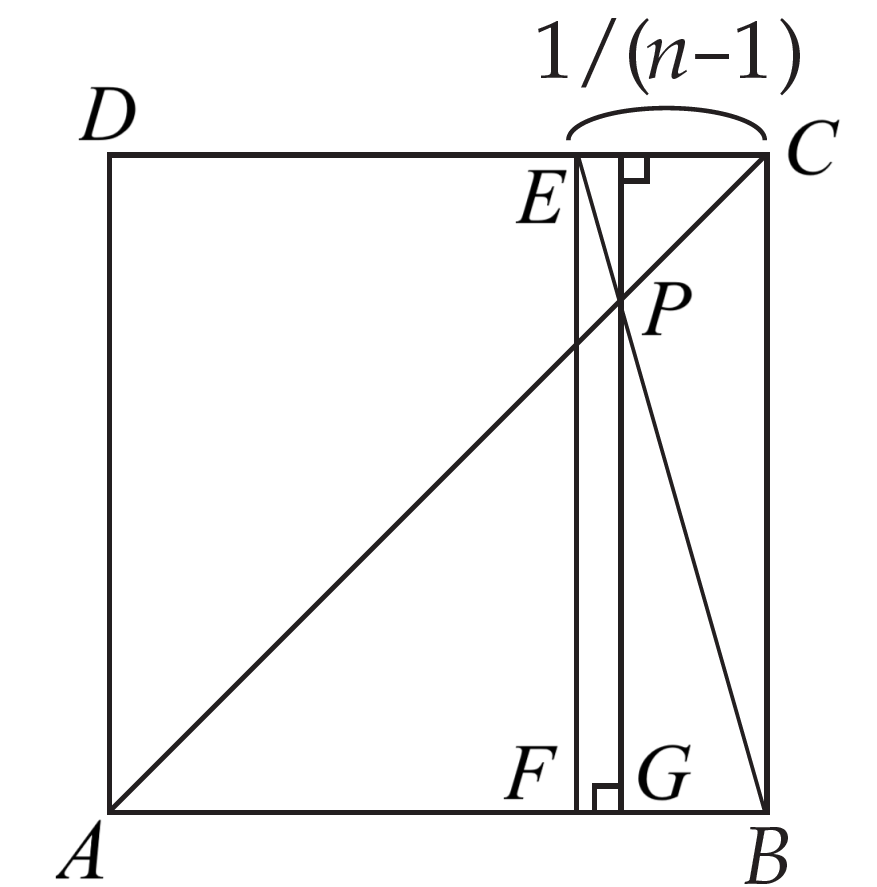
\includegraphics[width=0.3\textwidth]{images/razdelitev_stranice_n1.png}
    \caption[Metoda križajočih diagonal]{Konstrukcija po metodi križajočih se diagonal za splošen $n$. Vzeto in preurejeno iz~\cite[str. 38]{hull2013}.}
    \label{fig:razdelitev_stranice_n1}
\end{figure}

\begin{dokaz}
    Za $n = 1$ in $n = 2$ ni kaj dokazovati -- v prvem primeru pregiba sploh ni, v drugem primeru stranico prepolovimo.

    \textit{Baza indukcije:} Po trditvi~\ref{trd:kriz_diag_3} že vemo, da trditev drži za $n = 3$ (tudi za $5$).

    \textit{Indukcijska predpostavka:} Predpostavimo, da znamo stranico razdeliti na $n-1$ enakih delov.

    \textit{Indukcijski korak:} Dokazujemo, da znamo stranico razdeliti na $n$ enakih delov. Po navodilih za konstrukcijo iz trditve konstruiramo točko $P$ in pri tem označimo še točke $E, F$ in $G$, kot kaže slika~\ref{fig:razdelitev_stranice_n1}. Potem je dokaz posplošena različica tistega za trditev~\ref{trd:kriz_diag_3}:
    \begin{enumerate}
        \item \textit{Analitičen pristop:} Naj bo oglišče $A$ koordinatno izhodišče in oglišče $B$ točka $(1, 0)$. Premica, ki je nosilka diagonale $AC$, ima tako enačbo $y = x$, nosilka diagonale $CE$ pa $y = -(n-1)x + (n-1)$. Točka $P$ je njuno presečišče in ima tako koordinate $((n-1)/n, (n-1)/n)$. Torej je od desne stranice kvadrata res oddaljena za $1/n$.
        \item \textit{Preko podobnih trikotnikov:} Trikotnik $\triangle AGP$ je enakokrak in naj bo $|AG| = |GP| = x$. Iz razmerij dolžin stranic podobnih trikotnikov $\triangle EFB$ in $\triangle PGB$ sledi
        \begin{align*}
            \frac{|EF|}{|FB|} &= \frac{|PG|}{|GB|}, \\
            \frac{1}{\frac{1}{n-1}} &= \frac{x}{1 - x}, \\
            x &= \frac{n-1}{n}.
        \end{align*}
        Točka $P$ je od desne stranice kvadrata res oddaljena za $1-x = 1/(n + 1)$.
    \end{enumerate}
\end{dokaz}

\begin{posledica}
    Poljubno daljico znamo razdeliti na $n$ skladnih delov za vsak $n \in \N$.
\end{posledica}

\begin{dokaz}
    Vzemimo neko daljico poljubne dolžine. Ker znamo konstruirati pravokotnice skozi točke in prenašati razdalje, lahko konstruiramo kvadrat, katereda zgornja stranica dana daljica. Po zgornji trditvi jo znamo razdeliti v razmerju $(n-1) : 1$ za vsak $n \in \N$. Potem moramo njen daljši del razdeliti na $n-1$ skladnih delov. To storimo na enak način kot prej -- konstruiramo manjši kvadrat s to novo stranico in ponovimo postopek. Ustavimo se, ko na nekem koraku stranico kvadrata razdelimo v razmerju $1:1$ (slika~\ref{fig:razdelitev_daljice_n1}). Takrat bo zgornja stranica oz. dana daljica razdeljena na $n$ skladnih delov.
\end{dokaz}

\begin{figure}[h]
    \centering
    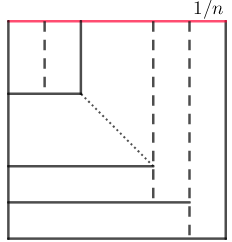
\includegraphics[width=0.3\textwidth]{images/razdelitev_daljice_n1.png}
    \caption[Razdelitev daljice na enake dele]{Razdelitev poljubne stranice (označena z rdečo) na poljubno število skladnih delov.}
    \label{fig:razdelitev_daljice_n1}
\end{figure}

\subsubsection*{Metoda po posplošenem prvem Hagovem izreku}
\label{podpogl:razdelitev_hag1_spl}

Spomnimo se prvega Hagovega izreka, kjer nam prepogib oglišča $B$ na središče daljice $CD$ v točki $H$ na daljici $AD$ povzroči njeno razdelitev v razmerju $2:1$. Nato smo izrek posplošili in namesto središča zgornje stranice izbrali poljubno točko, ki je za $x$ odmaknjena od oglišča $C$ (slika~\ref{fig:hagov_izrek1_splosen}). Pri tem smo med drugim izračunali razdaljo $y_2 = |HA| = 2x/(1+x)$.

Razveseli nas, da pri $x = 1/n$ dobimo ravno $y_2 = 2/(n+1)$, kar je dvakratnik števila $1/(n+1)$. Če torej znamo zgornjo stranico razdeliti v razmerju $(n-1):1$, nam središče daljice $|HA|$ levo stranico razdeli v razmerju $n:1$. Na sliki~\ref{fig:razdelitev_daljice_h1} je prikaz za $n = 2, 3, 4$ in splošen $n$ (pri tem se sicer na zgornjo stranico prepogne spodnje levo oglišče, zato je to zrcalna različica slike, kot smo je vajeni). Po indukciji (prvi Hagov izrek je baza indukcije pri $n=2$) je to še ena metoda za razdelitev daljice na poljubno število skladn95ih delov preko prepogibanja kvadratnega lista papirja.

\begin{figure}[h]
    \centering
    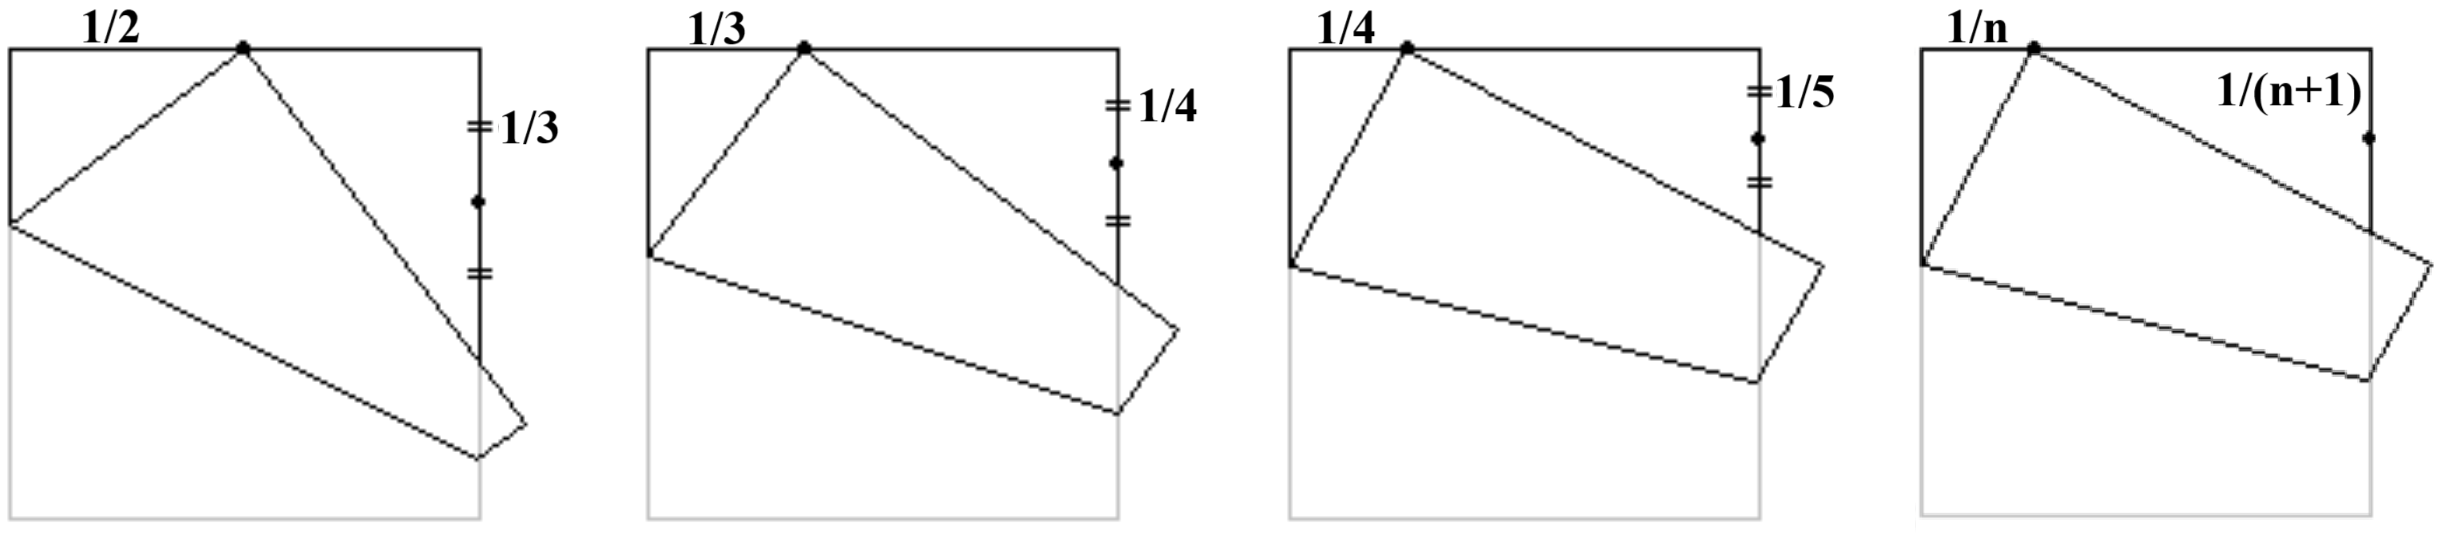
\includegraphics[width=\textwidth]{images/razdelitev_daljice_h1.png}
    \caption[Razdelitev na enake dele (prvi Hagov izrek)]{Konstrukcije razmerij po posplošenem prvem Hagovem izreku.}
    \label{fig:razdelitev_daljice_h1}
\end{figure}

\subsubsection*{Metoda3}

\subsubsection*{Metoda4}

\textcolor{red}{Več metod (vsaj tri?), Hull2013 (str.\ 36--40).}

\textcolor{red}{Do zdaj smo imeli metode z razdelitvijo preko prepogibanja kvadratnega lista papirja. Za razdelitev preko pravokotnika pa glej~\cite[str.\ 107--134]{haga2008}.}

\subsection{$X$-pregibi}

\textcolor{red}{Glej~\cite[str.\ 33--44]{haga2008}}


\subsection{Reševanje nerešljivih starogrških problemov}
\label{podpogl:starogrskiproblemi}

Z evklidskimi konstrukcijami se je seveda pojavilo konstruktibilnih ugank -- vprašanj, ali je specifično število konstruktibilno (in na kakšnen način) ali ne. Zelo znani so trije t.\ i.\ ``starogrški' problemi, ki so matematike bremenili več kot tisočletje, začenši s časom Evklida (300 pr.\ Kr.), končno pa sta nanje dokončno odgovorila Niels Henrik Abel (1802--1829) in Evariste Galois (1811--1832) v začetku 19.\ stoletja. Gre za sledeče tri probleme:
\begin{itemize}
    \item \textbf{Podvojitev kocke} Imejmo že konstruktibilno kocko. Konstruiraj novo kocko, ki ima dvakrat večji volumen od prve (problem se poenostavi na iskanje konstrukcije števila $\sqrt[3]{2}$).
    \item \textbf{Trisekcija kota} Dan je poljuben konstruktibilen kot. Konstruiraj kot, ki prvega deli na tri skladne dele.
    \item \textbf{Kvadratura kroga} Za dan konstruktibilen krog konstruiraj kvadrat, ki ima enako ploščino kot dani krog (problem se poenostavi na konstrukcije števila $\sqrt{\pi}$).
\end{itemize}

Z znanjem, ki sta ga znanosti posredovala Abel in Galois, se da pokazati, da ti trije problemi z evklidskim orodjem niso rešljivi. V nalogi smo do sedaj že večkrat omenili, da pa obstajajo origami konstrukcije (celo več metod za isti problem!), ki nam konstruirajo kubični koren origami števila ter razdelijo kot na tri skladne dele. Vse metode, ki bodo sedaj naštete, zahtevajo uporabo Belochinega pregiba (operacije~\ref{op:O7}), kar je logično, saj so vse ostale origami operacije dovolj za vse evklidske konstrukcije. Žal pa tudi tu ostajamo nemočni glede konstrukcije števila $\sqrt{\pi}$, saj je transcedentno.

\subsubsection*{Konstrukcija števila $\sqrt{r}$}

Preden si pogledamo konstrukcijo kubičnega korena, vzemimo origami število $r \in \mathcal{O}$ in kosntruirajmo njegov kvadratni koren (postopek je vzet iz~\cite[str.\ 58]{hull2013}).

Imejmo točko $A (0, 1) $ in premico $y = -1$. Na ordinatni osi označimo točko $B (0, -r/4)$ in z operacijo~\ref{op:O6} skoznjo naredimo pregib, ki točko $A$ položi na premico $y = -1$. Njena zrcalna slika je $A' (t, 0) $ za nek $t \in \R$ (slika~\ref{fig:konstrukcija_korena}).

\begin{figure}[h]
    \centering
    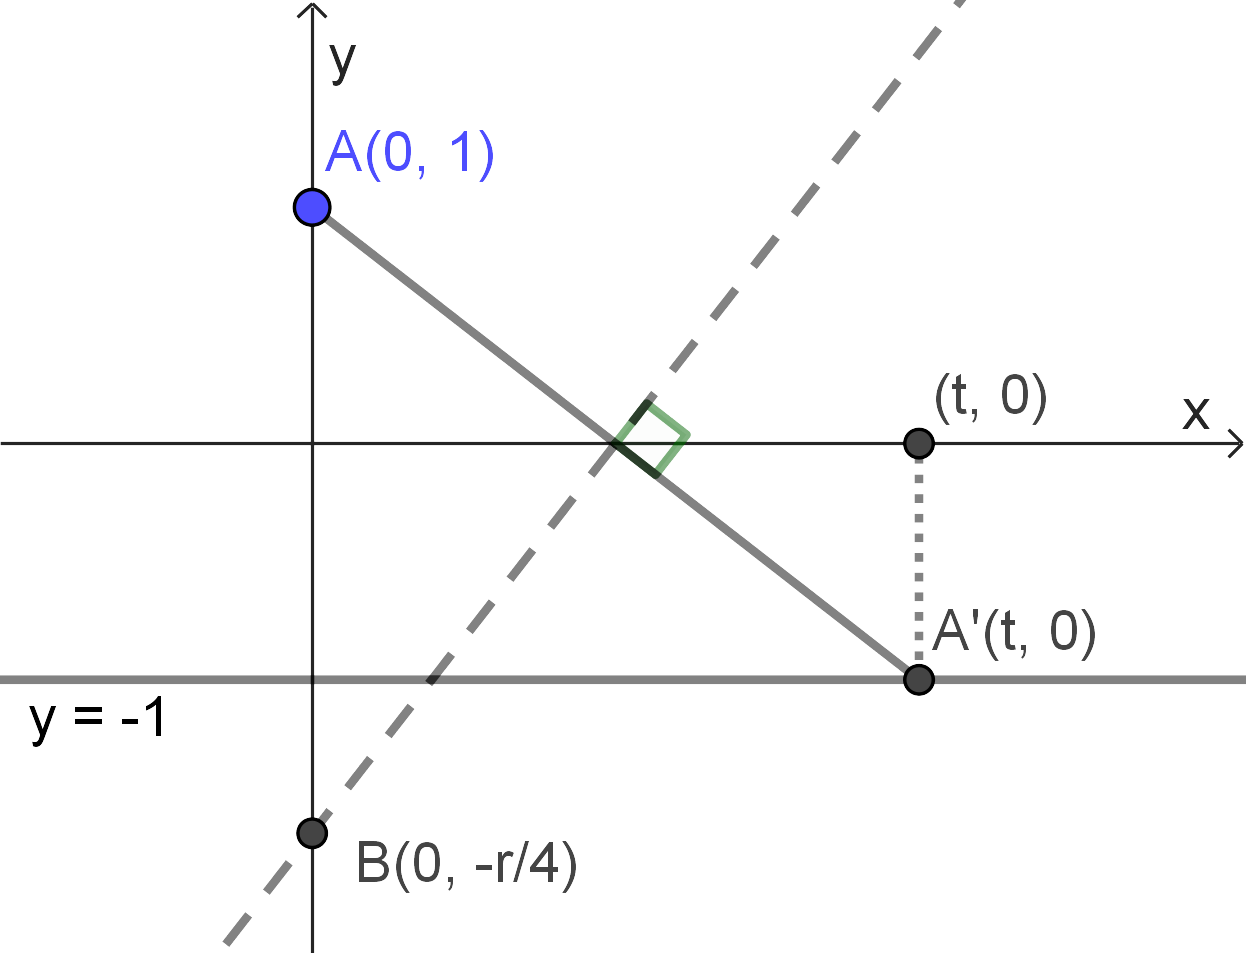
\includegraphics[width=0.5\textwidth]{images/kvadratni_koren.png}
    \caption[Konstrukcija korena]{Konstrukcija števila $\sqrt{r}$ za poljuben $r \in \Q^{+}$.}
    \label{fig:konstrukcija_korena}
\end{figure}

Pregib po konstrukciji poteka skozi točko $B$ in razpolovišče daljice $AA'$, torej je njegov koeficient $k_B = \frac{r}{2t}$ (izpeljavo prepuščamo bralcu). Ker je pregib simetrala daljice $AA'$, njena nosilka pa ima koeficient $k_A = - \frac{2}{t}$, dobimo
\begin{align*}
    k_B &= - \frac{1}{k_A},\\
    \frac{r}{2t} &= \frac{t}{2},\\
    r &= t^2 \text{ oz. } t = \sqrt{r}.
\end{align*}
Na koncu le še prepognemo pravokotnico na abscisno os skozi točko $A'$ in tako dobimo točko $(\sqrt{r}, 0)$. Torej smo konstruirali število $\sqrt{r}$ za poljuben $r \in \mathcal{O}$.

\subsubsection{Podvojitev kocke}
\label{podpogl:podvojitev_kocke}

Po legendi iz grške mitologije je bog Apolon po oraklju prebivalcem svojega rojstnega otoka Delosa sporočil, da mu morajo, če se želijo znebiti smrtonosne kuge, zgraditi nov oltar v obliki kocke, ki je enak prejšnjemu, le da mora biti dvakrat večji po prostornini. Torej je bilo potrebno konstruirati kocko s stranico, ki je za faktor $\sqrt[3][2]$ večja od stranice originalne kocke. Po drugi legendi pa naj bi Platon izjavil, da je ta problem, ki so ga prejeli na njegovi Akademiji v Atenah, poslan od bogov samih z namenom osramotiti Grke zaradi njihovega zanemarjanja in prezira do matematike (ker z evklidskim orodjem niso znali konstruirati poljubnih dolžin)~\cite[str.\ 29]{geometricconstructions}.

Ne vemo, ali so bili Grki prepričani, da se problema z neoznačenim ravnilom in šestilom ne da rešiti. Vsekako pa jim je manjkalo algebrsko znanje. Če je stranica kocke dolga $1$, je stranica podvojene kocke dolga $\sqrt[3]{2}$ in ker je obseg $\Q(\sqrt[3]{2})$ vektorski prostor razsežnosti $3$ nad obsegom $\Q$ (enačba $ x^3 - 2 = 0 $ nima racionalne rešitve), podvojitev kocke po izreku~\ref{izr:evkl_konstr} z evkliskim orodjem res ni mogoča~\cite[str. 78]{jerman1998}.

\subsubsection*{Starogrška rešitev preko presečišča dveh parabol}

Mogoče Grkom ni uspelo priti do tega premisleka, vendar so problem vseeno uspeli rešiti, čeprav po drugi poti; uporabili so še eno močno matematično orodje -- stožnice. Videla v~\cite{videla1997} dokaže izrek, ki je identičen izreku~\ref{izr:origami_konstr} (ki govori, katera števila so origami števila), le da namesto origamija uporabi stožnice. V bistvu s tem dokaže, da so origami kosntrukcije ekvivalentne konstrukcijam s stožnicami!

V istem viru Videla tudi navaja konstrukcijo s parabolami, ki za dano dolžino $a$ podajo dolžino $c$, za katero velja $c^3 = a$. Njen avtor je Menehmo (prb.\ 350 pr.\ Kr.), tutor Aleksandra Velikega. Vzel je sledeči paraboli (slika~\ref{fig:videla}):
\begin{itemize}
    \item $\mathcal{P}_1: y = x^2$ z goriščem v točki $(0, \frac{1}{4})$ in premico vodnico $y = - \frac{1}{4}$ in
    \item $\mathcal{P}_1: x = \frac{y^2}{a}$ z goriščem v točki $(\frac{a}{4}, 0)$ in premico vodnico $x = - \frac{a}{4}$.
\end{itemize}
\begin{figure}[h]
    \centering
    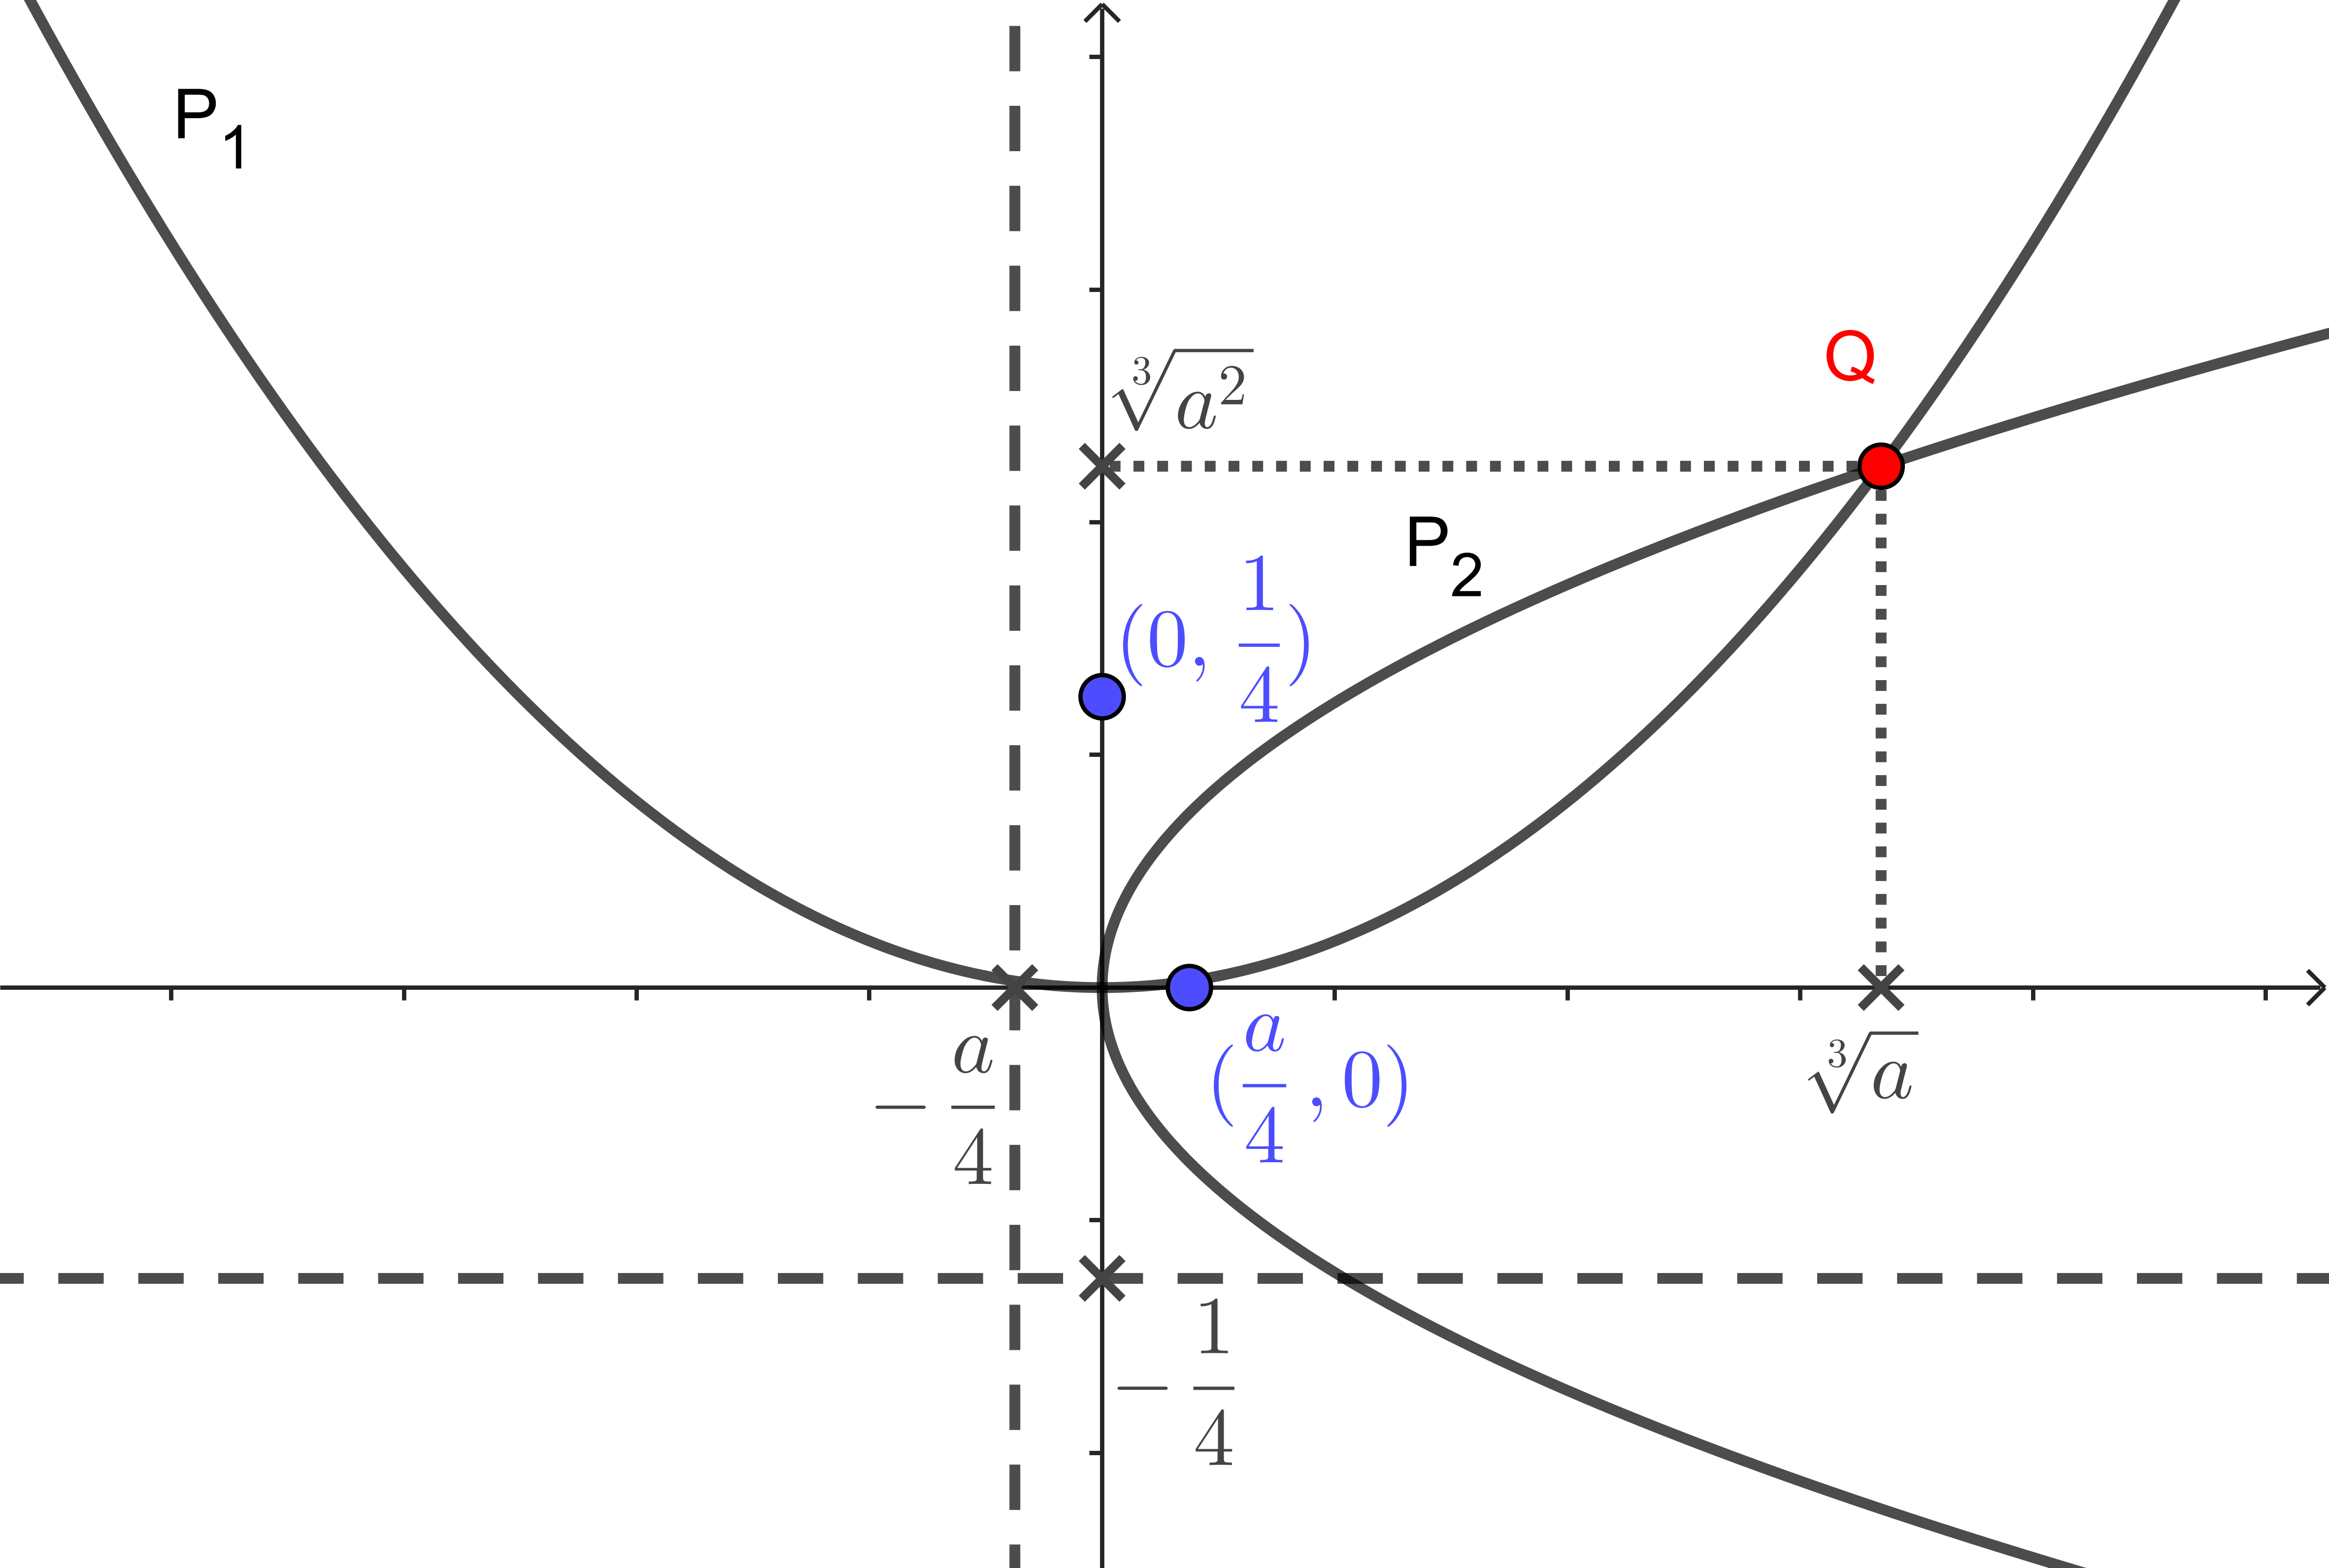
\includegraphics[width=0.7\textwidth]{images/starogr_problemi/cube_parabola.png}
    \caption[Menehmova konstrukcija kubičnega korena]{Menehmova konstrukcija števila $\sqrt[3]{2}$ preko parabol. Vzeto iz~\cite[str.\ 6]{videla1997}.}
    \label{fig:videla}
\end{figure}
Presečišči teh dveh parabol dobimo preko enakosti
$$y = x^2 = y^4/a^2,$$
kar nam da enačbo $y(a^2-y^3) = 0$ z rešitvama $y=0$ in $y = \sqrt[3]{a^2}$. Presečišči sta torej koordinatno izhodišče in točka $Q = (\sqrt[3]{a}, \sqrt[3]{a^2}) $. Njena abscisa je naša rešitev.
\opomba{Čeprav je konstrukcija enostavna in logična, je praktično težje izvedena, saj z roko ne znamo natančno risati parabol. \textcolor{red}{mal lepše to napiši. Pa bodi ziher da se ne da. Pač elipso se da mehanično.}}

\subsubsection*{Martinova konstrukcija}

George E.\ Martin v~\cite[str.\ 156--157]{geometricconstructions} poda preprosto konstrukcijo števila $\sqrt[3]{k}$ za poljubno origami število $k$. Tudi on pri tem uporabi dve paraboli, vendar pri postopku potrebujemo le njuni gorišči in premici vodnici. Ne bomo iskali njunih presečišč, temveč bomo z Belochinim pregibom konstruirali njuno skupno tangento, ki nam bo podala željeni rezultat.

Naj bo $k \in \mathcal{O}$ poljuben. Vzemimo paraboli z goriščema v točkah $P = (-1, 0)$ in $Q = (0, -k)$ ter premici vodnici $p: x = 1$ in $q: y = k$. Paraboli imata skupno gorišče v koordinatnem izhodišču in sta pravokotni druga na drugo, torej imata eno samo skupno tangento. Prepognimo točko $P$ na premico $p$ in točko $Q$ na premico $q$. Pregib seka $y$-os v točki $R$ (slika~\ref{fig:martin}).
\begin{figure}[h]
    \centering
    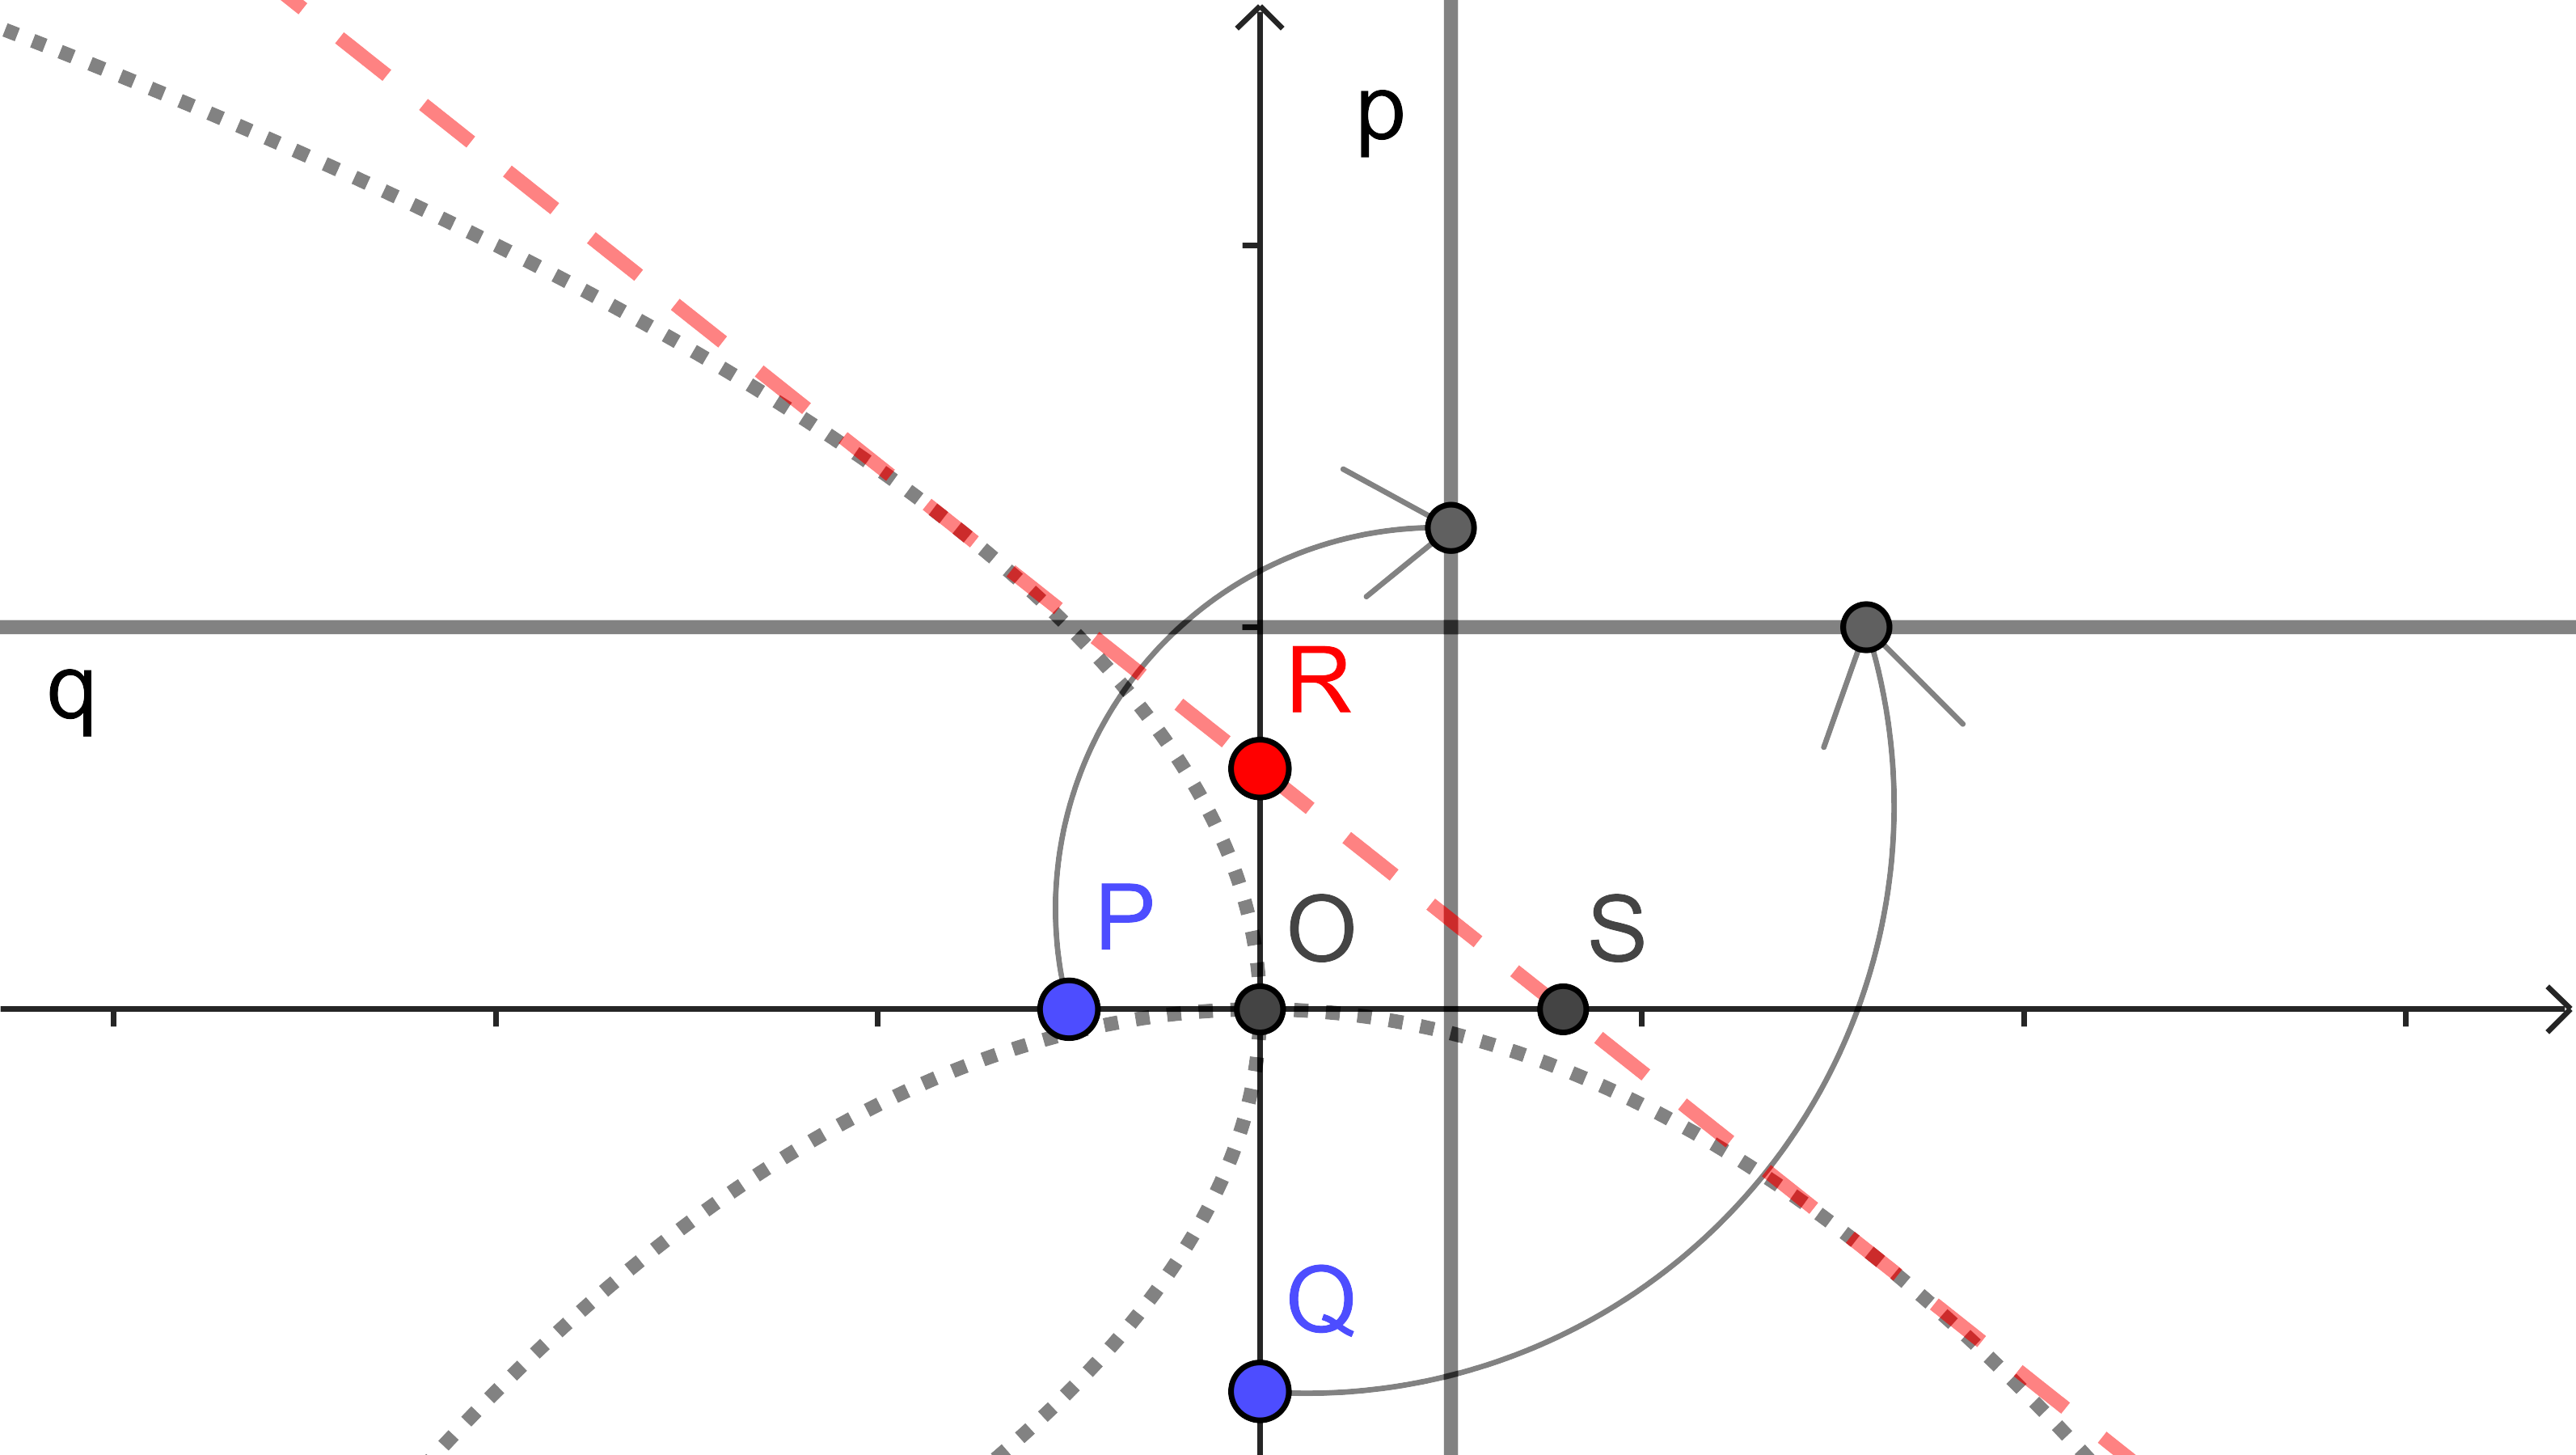
\includegraphics[width=0.6\textwidth]{images/starogr_problemi/cube_martin.png}
    \caption[Martinova konstrukcija kubičnega korena]{Martinova konstrukcija števila $\sqrt[3]{k}$.}
    \label{fig:martin}
\end{figure}
\begin{trditev}
    Točka $R$ iz zgornje konstrukcije ima koordinate $(0, \sqrt[3]{k})$.
\end{trditev}
\begin{dokaz}
    Označimo z $O$ koordinatno izhodišče in s $S$ presečišče pregiba z $x$-osjo. Točki $R$ in $S$ sta zaradi take izbire gorišč in premic vodnic ravno središči daljic z enim krajiščem v točkah $P$ in $Q$ ter drugim krajiščem v njunih slikah. Torej velja $PR \perp RS \perp SQ$. Zato so trikotniki $\triangle POR, \triangle ROS$ in $\triangle SOQ$ podobni. Iz tega ob upoštevanju $|OP| = 1$ in $|OQ| = k$ dobimo razmerje
    $$ \frac{|OR|}{|OP|} = \frac{|OS|}{|OR|} = \frac{|OQ|}{|OS|} \Longrightarrow |OR| = \frac{|OS|}{|OR|} = \frac{k}{|OS|}, $$
    iz česar sledi
    $$ |OR|^3 = |OR| \cdot \frac{|OS|}{|OR|} \cdot \frac{k}{|OS|} = k \Longrightarrow |OR| = \sqrt[3]{k}.$$
\end{dokaz}
\begin{opomba}
    V razdelku~\ref{podpogl:beloch_kvadrat_koren} bomo spoznali konstrukcijo števila $\sqrt[3]{2}$ preko Belochinega kvadrata, ki je v bistvu poseben primer Martinove konstrukcije.
\end{opomba}

\subsubsection*{Messerjeva konstrukcija}

Peter Messer v~\cite{messer1986} navaja avtorski postopek, ki sicer ne konstruira števila $\sqrt[3]{2}$ kot razdaljo, temveč kot razmerje: kvadraten list papirja po horizontali razdelimo na tri dele (to sedaj že znamo storiti) ter točki $p_1$ in $p_2$ s prepogibom položimo na premici $L_1$ in $L_2$, kot kaže slika~\ref{fig:messer} (levo).
\begin{figure}[h]
    \centering
    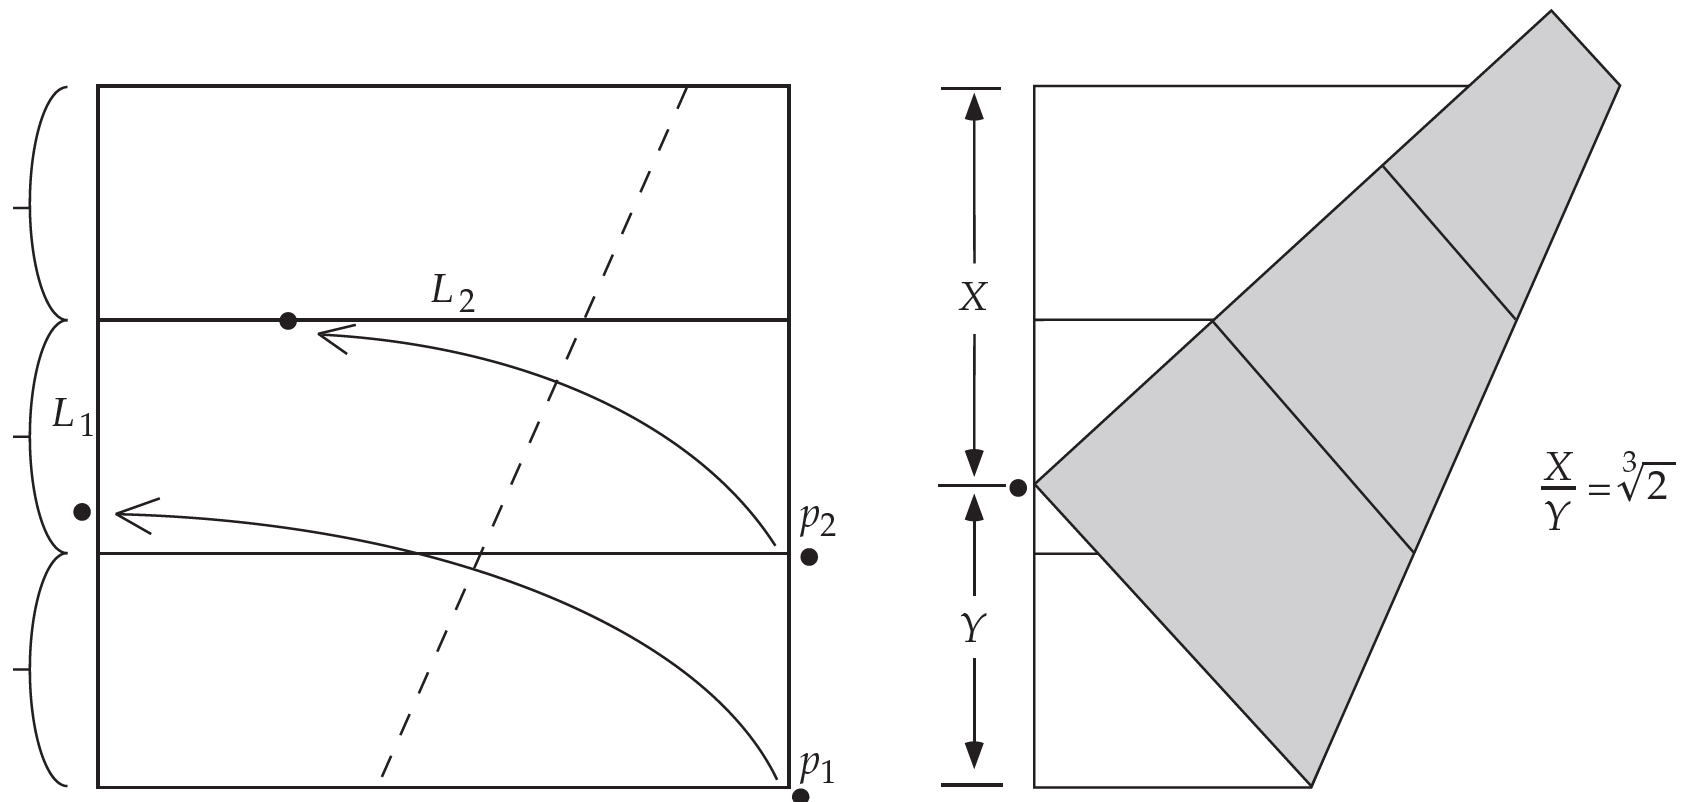
\includegraphics[width=0.68\textwidth]{images/starogr_problemi/messer1.png}
    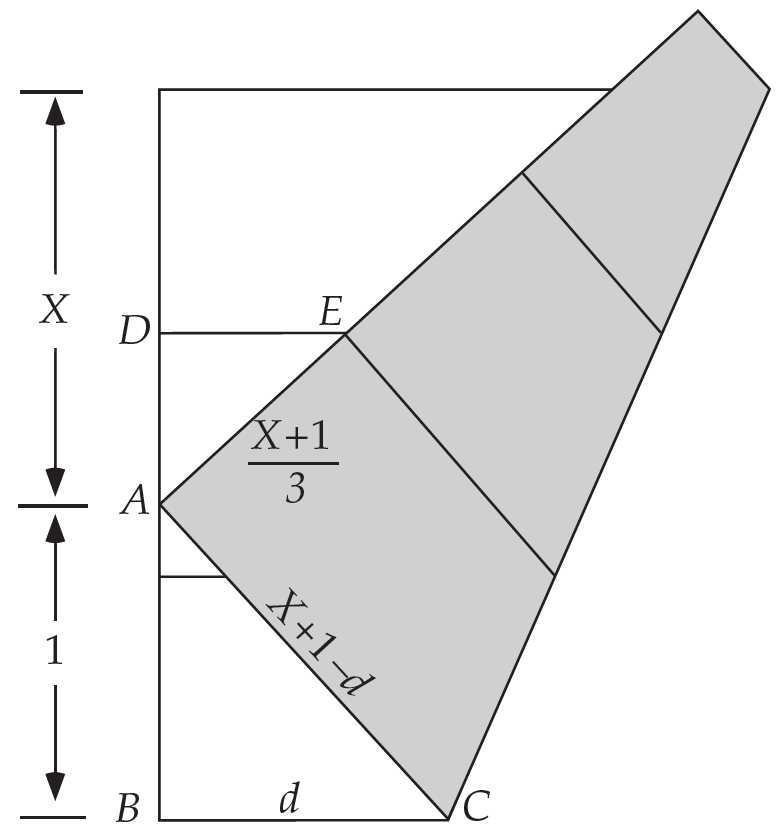
\includegraphics[width=0.3\textwidth]{images/starogr_problemi/messer2.png}
    \caption[Messerjeva konstrukcija]{Messerjeva konstrukcija razmerja $\sqrt[3]{2}$. Vzeto iz~\cite[str.\ 67--68]{hull2013}.}
    \label{fig:messer}
\end{figure}
\begin{trditev}
    Slika točke $p_1$ deli levo stranico kvadrata v razmerju $\sqrt[3]{2}$.
\end{trditev}
\begin{dokaz}
    Vpeljimo oznake $X, Y, A, B, C, D, E$ ter $d = |BC|$, kot kaže slika~\ref{fig:messer}. Dokazati moramo $X/Y = \sqrt[3]{2}$, za lažje računanje pa brez škode privzemimo $Y=1$. Stranica kvadrata je tako dolga $X+1$, zato je $|AC| = X+1-d$ in $|AE| = (X+1)/3$.

    Opazimo podobna pravokotnika $\triangle ABC$ in $\triangle ADE$. Iz trikotnika $\triangle ABC$ s pomočjo Pitagorovega izreka izrazimo $d = (X^2+2X)/(2X+2)$, preko leve stranice pa še $|AD| = X - (X+1)/3 = (2X-1)/3$. Iz podobnosti omenjenih trikotnikov izrazimo razmerje katete in hipotenuze z enačbo $|BC|/|AC| = |AD|/|AE|$. Ko vstavimo noter vse vrednosti, odvisne od $X$, dobimo enačbo
    $$ \frac{X^2 + 2X}{X^2 + 2X + 2} = \frac{2X - 1}{X + 1},$$
    ki se nam poenostavi prav v $X^3 = 2$. Torej je $X = \sqrt[3]{2}$.
\end{dokaz}
\opomba{Lahko bi rekli, da poleg razmerja v primeru $Y=1$ Messer konstruira razdaljo $\sqrt[3]{2}$, vendar je razdalja $Y$ odvisna od stranice kvadrata. V tem primeru bi morali vzeti kvadraten list papira s stranico $1 + \sqrt[3]{2}$, za kar bi pač potrebovali že konstrukcijo kubičnega korena števila $2$. Da bi pri splošnem kvadratnem listu papirja dobili to dolžino, moramo razdalji $X$ in $Y$ z origamijem še deliti, to pa že znamo.}

\subsubsection{Trisekcija kota}
\label{podpogl:trisekcija}

Kot $90^\circ$ znamo tretjiniti z neoznačenim ravnilom in šestilom, saj znamo konstruirati kot $30^\circ$. Težava je, da ne obstaja konstrukcija, s katero na tri skladne kote razdelimo \emph{poljuben} kot. V~\cite[str.\ 77--78]{jerman1998} je dokaz o neobstoju konstrukcije za trisekcijo kota $60^\circ$. Avtor se pri tem sklicuje na izrek~\ref{izr:evkl_konstr} in opombo~\ref{op:razseznost_obsega_evkl} iz razdelka~\ref{podpogl:evkl_konstruktibilnost}. Na kratko -- iz zveze $ 1/2 = \cos 60^\circ = \cos(3 \cdot 20^\circ) = 4 \cos^3 20^\circ - 3 \cos 20^\circ, $ z zamenjavo $x = \cos 20^\circ$ dobimo enačbo $8 x^3 - 6x - 1 = 0$, ki nima racionalne rešitve. Razsežnost prostora $\Q(x)$ nad obsegom $\Q$ je tako enaka $3$ in števila $ \cos 20^\circ $ se ne da narisati le z ravnilom in šestilom. Zato trisekcija z evklidskim orodjem v splošnem ni mogoča.

% SPODNJI DOKAZ JE PREPISAN IZ VIRA IN SAMO CITIRAN V prejšnjem odstavku

% Algebraični dokaz, da z evklidskim orodjem ne moremo tretjiniti poljubnega kota -- dokažimo za kot $60°$. (iz~\cite[str.\ 77--78]{jerman1998})

% Kot $60°$ znamo narisati. Če bi ga znali razdeliti na tri enake dele, bi potemtake znali narisati tudi kot $20°$, s tem pa (ker znamo risati pravokotnice) tudi $\cos 20°$ \textcolor{red}{slika z enotsko krožnico}. Pokažimo, da to ne gre.

% Izračunajmo minimalni polinom števila $\cos 20°$. Ker je
% $$ \frac{1}{2} = \cos 60° = \cos(3 \cdot 20°) = 4 \cos^3 20° - 3 \cos 20°, $$
% ima polinom $ p(x) = 8 x^3 - 6x - 1 $ ničlo $ \cos 20°$. Minimalni polinom števila $ \cos 20°$ deli polinom $p$. Če polinom $p$ razpade na produkt dveh polinomov s koeficienti v $\Q$, je eden od polinomov zagotovo linearen. To pa bi pomenilo, da ima polinom $p$ vsaj eno racionalno ničlo. Edini kandidatki za racionalne ničle polinoma $p$ so števila iz množice
% $$ \{\pm 1, \pm \frac{1}{2}, \pm \frac{1}{4}, \pm \frac{1}{8} \}. $$ Nobeno od teh števil ni ničla polinoma $p$, zato se $p$ ne da razcepiti na produkt dveh polinomov z racionalnimi koeficienti. Minimalni polinom števila $ \cos 20°$ je torej enaka
% $$ m(x) = \frac{1}{8} p(x) = x^3 - \frac{3}{4} x - \frac{1}{8}. $$
% Tako je razsežnost prostora $\Q(\cos 20°)$  nad obsegom $\Q$ enaka $3$ in števila $ \cos 20° $ se ne da narisati le z ravnilom in šestilom.

% Zato trisekcija kota v splošnem ni mogoča.

\subsubsection*{Starogrška rešitev preko presečišča krožnice in hiperbole}

Grki so tudi ta problem uspeli rešiti s stožnicami. Videla v~\cite[str.\ 6--7]{videla1997} opisuje Pappusovo konstrukcijo iz $3$.\ stoletja po Kr., ki je tu ne bomo dokazali. Gre za sledeč postopek: Na kraku $BA$ poljubnega kota $\angle ABC$ izberemo poljubno točko $F$ in zarišemo krožnico s središčem v točki $B$ in polmerom $BF$. Naj bo $BD$ simetrala kota $\angle ABC$. Naj bo presečišče krožnice in hiperbole z ekscentičnostjo $2$, ki ima gorišče v točki $F$ in premico vodnico $BD$, točka $E$ (slika~\ref{fig:trisection_gr}). Potem poltrak $BE$ tretjini kot $\angle ABC$.

\begin{figure}[h]
    \centering
    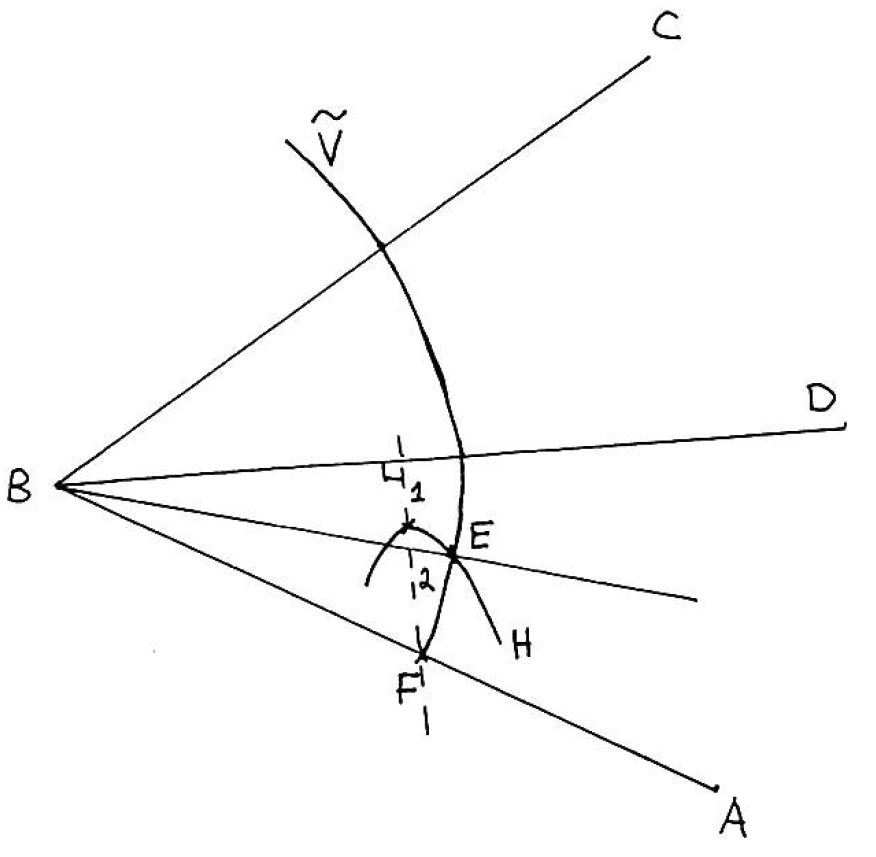
\includegraphics[width=0.6\textwidth]{images/starogr_problemi/trisection_grska.png}
    \caption[Pappusova trisekcija kota]{Pappusova trisekcija kota preko stožnic. Vzeto iz~\cite[str.\ 7]{videla1997}.}
    \label{fig:trisection_gr}
\end{figure}

\subsubsection*{Abejeva metoda}

Sledeča metoda ima ime po japonskemu matematiku Hisashiju Abeju, ki jo je odkril v $80$-ih letih prejšnjega stoletja. Postopek vključuje Belochin pregib, torej se ga ne da izvesti z evklidskim orodjem, edina pomankljivost metode pa je, da deluje le za ostre kote. Postopek je sledeč:

\begin{enumerate}
    \item Na kvadratnem listu papirja konstruiramo poljuben kot $\theta$, ki ima vrh v spodnjem desnem vogalu in en krak na spodnji stranici. Nato konstruiramo še dva horizontalna in ekvidistančna pregiba na dnu papirja (slika~\ref{fig:abe_1} levo).
    \item Točko $p_1$ prepognemo na spodnji horizontalen pregib, označen $L_1$, točko $p_2$ pa na poševen krak kota, označen z $L_2$ (slika~\ref{fig:abe_1} na sredi).
    \item Preden pregib razgrnemo, podaljšamo pregib $L_1$ do konca in nov pregib označimo z $L_3$ (slika~\ref{fig:abe_1} desno).
    \item Papir razgrnemo in tokrat v spodnji levi kot podaljšamo pregib $L_3$.
\end{enumerate}
\begin{figure}[h]
    \centering
    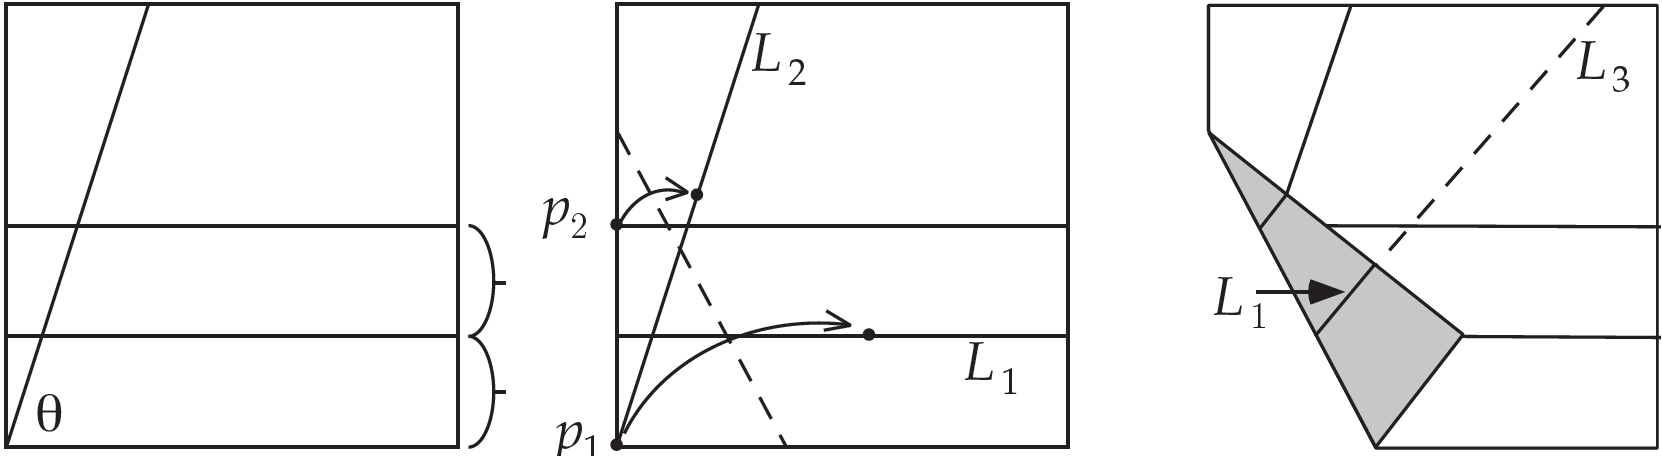
\includegraphics[width=0.95\textwidth]{images/starogr_problemi/abe_nastavek1.png}
    \caption[Abejeva metoda ($1$.\ del)]{Trisekcija kota po Abejevi metodi. Vzeto iz~\cite[str.\ 64]{hull2013}.}
    \label{fig:abe_1}
\end{figure}

\opomba{V $3$.\ koraku opravimo pregib še preden smo razgrnili prvega. To je za nas načeloma prepovedana poteza, vendar bi se dalo $L_3$ konstruirati tudi po klasični poti z enkratnimi prepogibi -- označili bi sliko točke, ki leži hkrati na $L_1$ in levi stranici kvadrata, ter točko v pregibu iz $2$.\ koraka, ki leži na $L_1$ in skozinju naredili pregib $L_3$ -- zato zaradi lažje izvedbe brez škode dopustimo tak postopek.}

\begin{trditev}
    Pregib $L_3$ poteka skozi točko $p_1$. Kot s krakoma $L_2$ in $L_3$ ter vrhom v točki $p_1$ je velik $\theta/3$.
\end{trditev}
\begin{posledica}
    Ko spodnji rob kvadrata prepognemo na pregib $L_3$, razdelimo kot $\theta$ na tri skladne kote.
\end{posledica}

\begin{dokaz}
    Posledica logično sledi, zato dokazujemo le trditev. Označimo z $x$ točko, ki leži na presečišču pregiba $L_1$ in pregiba iz $2$.\ koraka Abejeve metode. Z $A, B$, in $C$ označimo še slike točk z leve stranice kvadrata, kot kaže slika~\ref{fig:abe_2}.
    \begin{figure}[h]
        \centering
        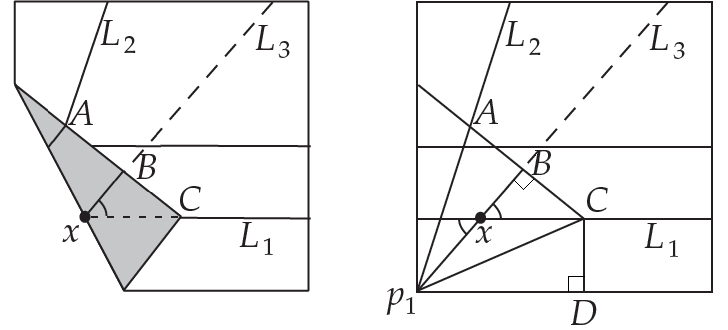
\includegraphics[width=0.7\textwidth]{images/starogr_problemi/abe_trisekcija.png}
        \caption[Abejeva metoda ($2$.\ del)]{Dokazovanje Abejeve metode. Vzeto in predelano iz~\cite[str.\ 65]{hull2013}.}
        \label{fig:abe_2}
    \end{figure}
    Ker je točka $C$ slika točke $p_1$ in $x$ leži na $L_1$, daljica $xC$ leži na $L_1$. Po konstrukciji daljica $xB$ leži na $L_3$, zato sta kota ob $x$, ko papir razgrnemo, skladna. Zaradi sovršnosti kotov daljica $p_1x$ leži na $L_3$, s čimer je prvi del trditve dokazan.
    
    Na razgrnjenem papirju zarišemo (ali prepognemo) še nekaj daljic (slika~\ref{fig:abe_2} desno). Ker velja $|AB| = |BC| = |CD|$ in imata pravokotna trikotnika $\triangle p_1AB$ in $\triangle p_1BC$ skupno še drugo kateto, trikotnika $\triangle p_1BC$ in $\triangle p_1CD$ pa skupno hipotenuzo, so vsi trije trikotniki skladni z enakim kotom v točki $p_1$, torej nam pregiba skozi daljici $p_1B$ (kar je ravno $L_3$) in $p_1C$ kot $\theta$ razdelijo na tri skladne kote.
\end{dokaz}

Ker ta postopek deluje le za ostre kote, si poglejmo naslednjo metodo, ki jo lahko uporabljamo tako za ostre kot tudi tope kote.

\subsubsection*{Justinova metoda}

Francoski matematik Jacques Justin za svojo metodo trisekcije ne zahteva kvadratnega lista papirja, ampak je dovolj kakršenkoli list. Lang v~\cite[str.\ 34]{lang2013} takole navaja njegovo kosntrukcijo:

Na sredo narišemo poljuben kot $\angle ABC$ (oster ali top) in njuna kraka podaljšamo skozi vrh $B$. Skozi vrh tudi konstruiramo poltrak, pravokoten na krat $BA$. Točko $C$ prezrcalimo čez vrh v točko $D$ ter nato obe točki prepognemo na nosilko kraka $BA$ in pravokotnico, kot kaže slika~\ref{fig:justin} (levo). Nazadnje na Belochin pregib konstruiramo še pravokotnico skozi točko $B$.
\begin{figure}[h]
    \centering
    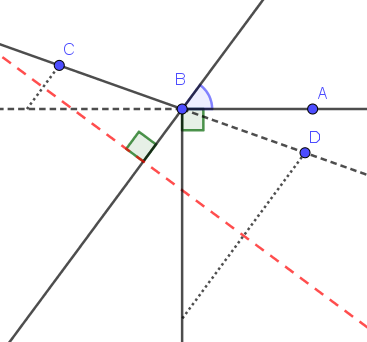
\includegraphics[width=0.45\textwidth]{images/starogr_problemi/justin_trisection.png}
    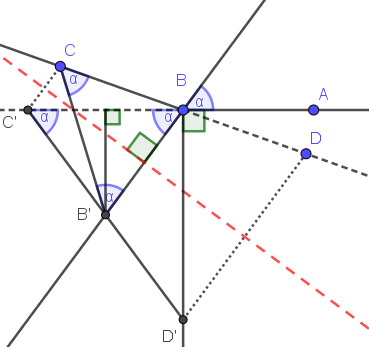
\includegraphics[width=0.45\textwidth]{images/starogr_problemi/justin_trisection_dokaz.png}
    \caption[Justinova trisekcija kota]{Justinova trisekcija kota (levo) in njen geometrijski dokaz (desno).}
    \label{fig:justin}
\end{figure}

\begin{trditev}
    Kot, ki v točki $B$ oklepata zadnja pravokotnica iz zgornje konstrukcije in krak $BA$, je tretjina kota $\angle ABC$.
\end{trditev}
\begin{dokaz}
    Označimo z $\alpha$ kot iz trditve. Naj bosta točki $C'$ in $D'$ sliki točk $C$ in $D$, točka $B'$ pa presečišče daljice $C'D'$ s pravokotnico iz trditve. Po konstrukciji Belochinega pregiba je daljica $C'D'$ slika daljice $CD$, torej je točka $B'$ slika točke $B$. Točka $B'$ je tako središče daljice $C'D'$ in zato je vzporednica k poltraku $BD'$ skozi točko $B'$ simetrala daljice $C'B$. Trikotnik $\triangle C'B'B$ je tako enakokrak in velja $\angle C'BB' = \angle B'C'B = \alpha$.
    
    Ker sta trikotnika $\triangle C'B'B$ in $\triangle CBB'$ zaradi simetričnosti glede Belochin pregib skladna, velja tudi $\angle B'CB = \angle CB'B = \alpha$. Iz vsote notranjih kotov trikotnike $\triangle CB'B$ sledi $\angle C'BC = 180^\circ - 3\alpha$, torej je $\angle ABC = 180^\circ - \angle C'BC = 3\alpha$. 
\end{dokaz}

\subsubsection*{Martinovi konstrukciji za trisekcijo ostrega kota}

George E.\ Martin v~\cite[poglavje 10]{geometricconstructions} navaja še dve metodi za trisekcijo ostrega kota.

Pri prvi vzamemo oster kot $\angle PQR$ in s točko $M$ označimo središče daljice $PQ$. Skozi $M$ konstruiramo pravokotnico $p$ na $QR$, nato pa še pravokotnico na $p$. Opravimo tisti Belochin pregib (od treh možnih), ki seka daljico $PM$ in točko $Q$ položi na premico $q$ (v točko $Q'$), točko $P$ pa na premico $p$ (v točko $P'$). S $T$ označimo presečišče daljice $QQ'$ s premico $p$ in s $S$ presečišče pregiba s premico $q$ (slika~\ref{fig:trisection_10.4}).

\begin{figure}[h]
    \centering
    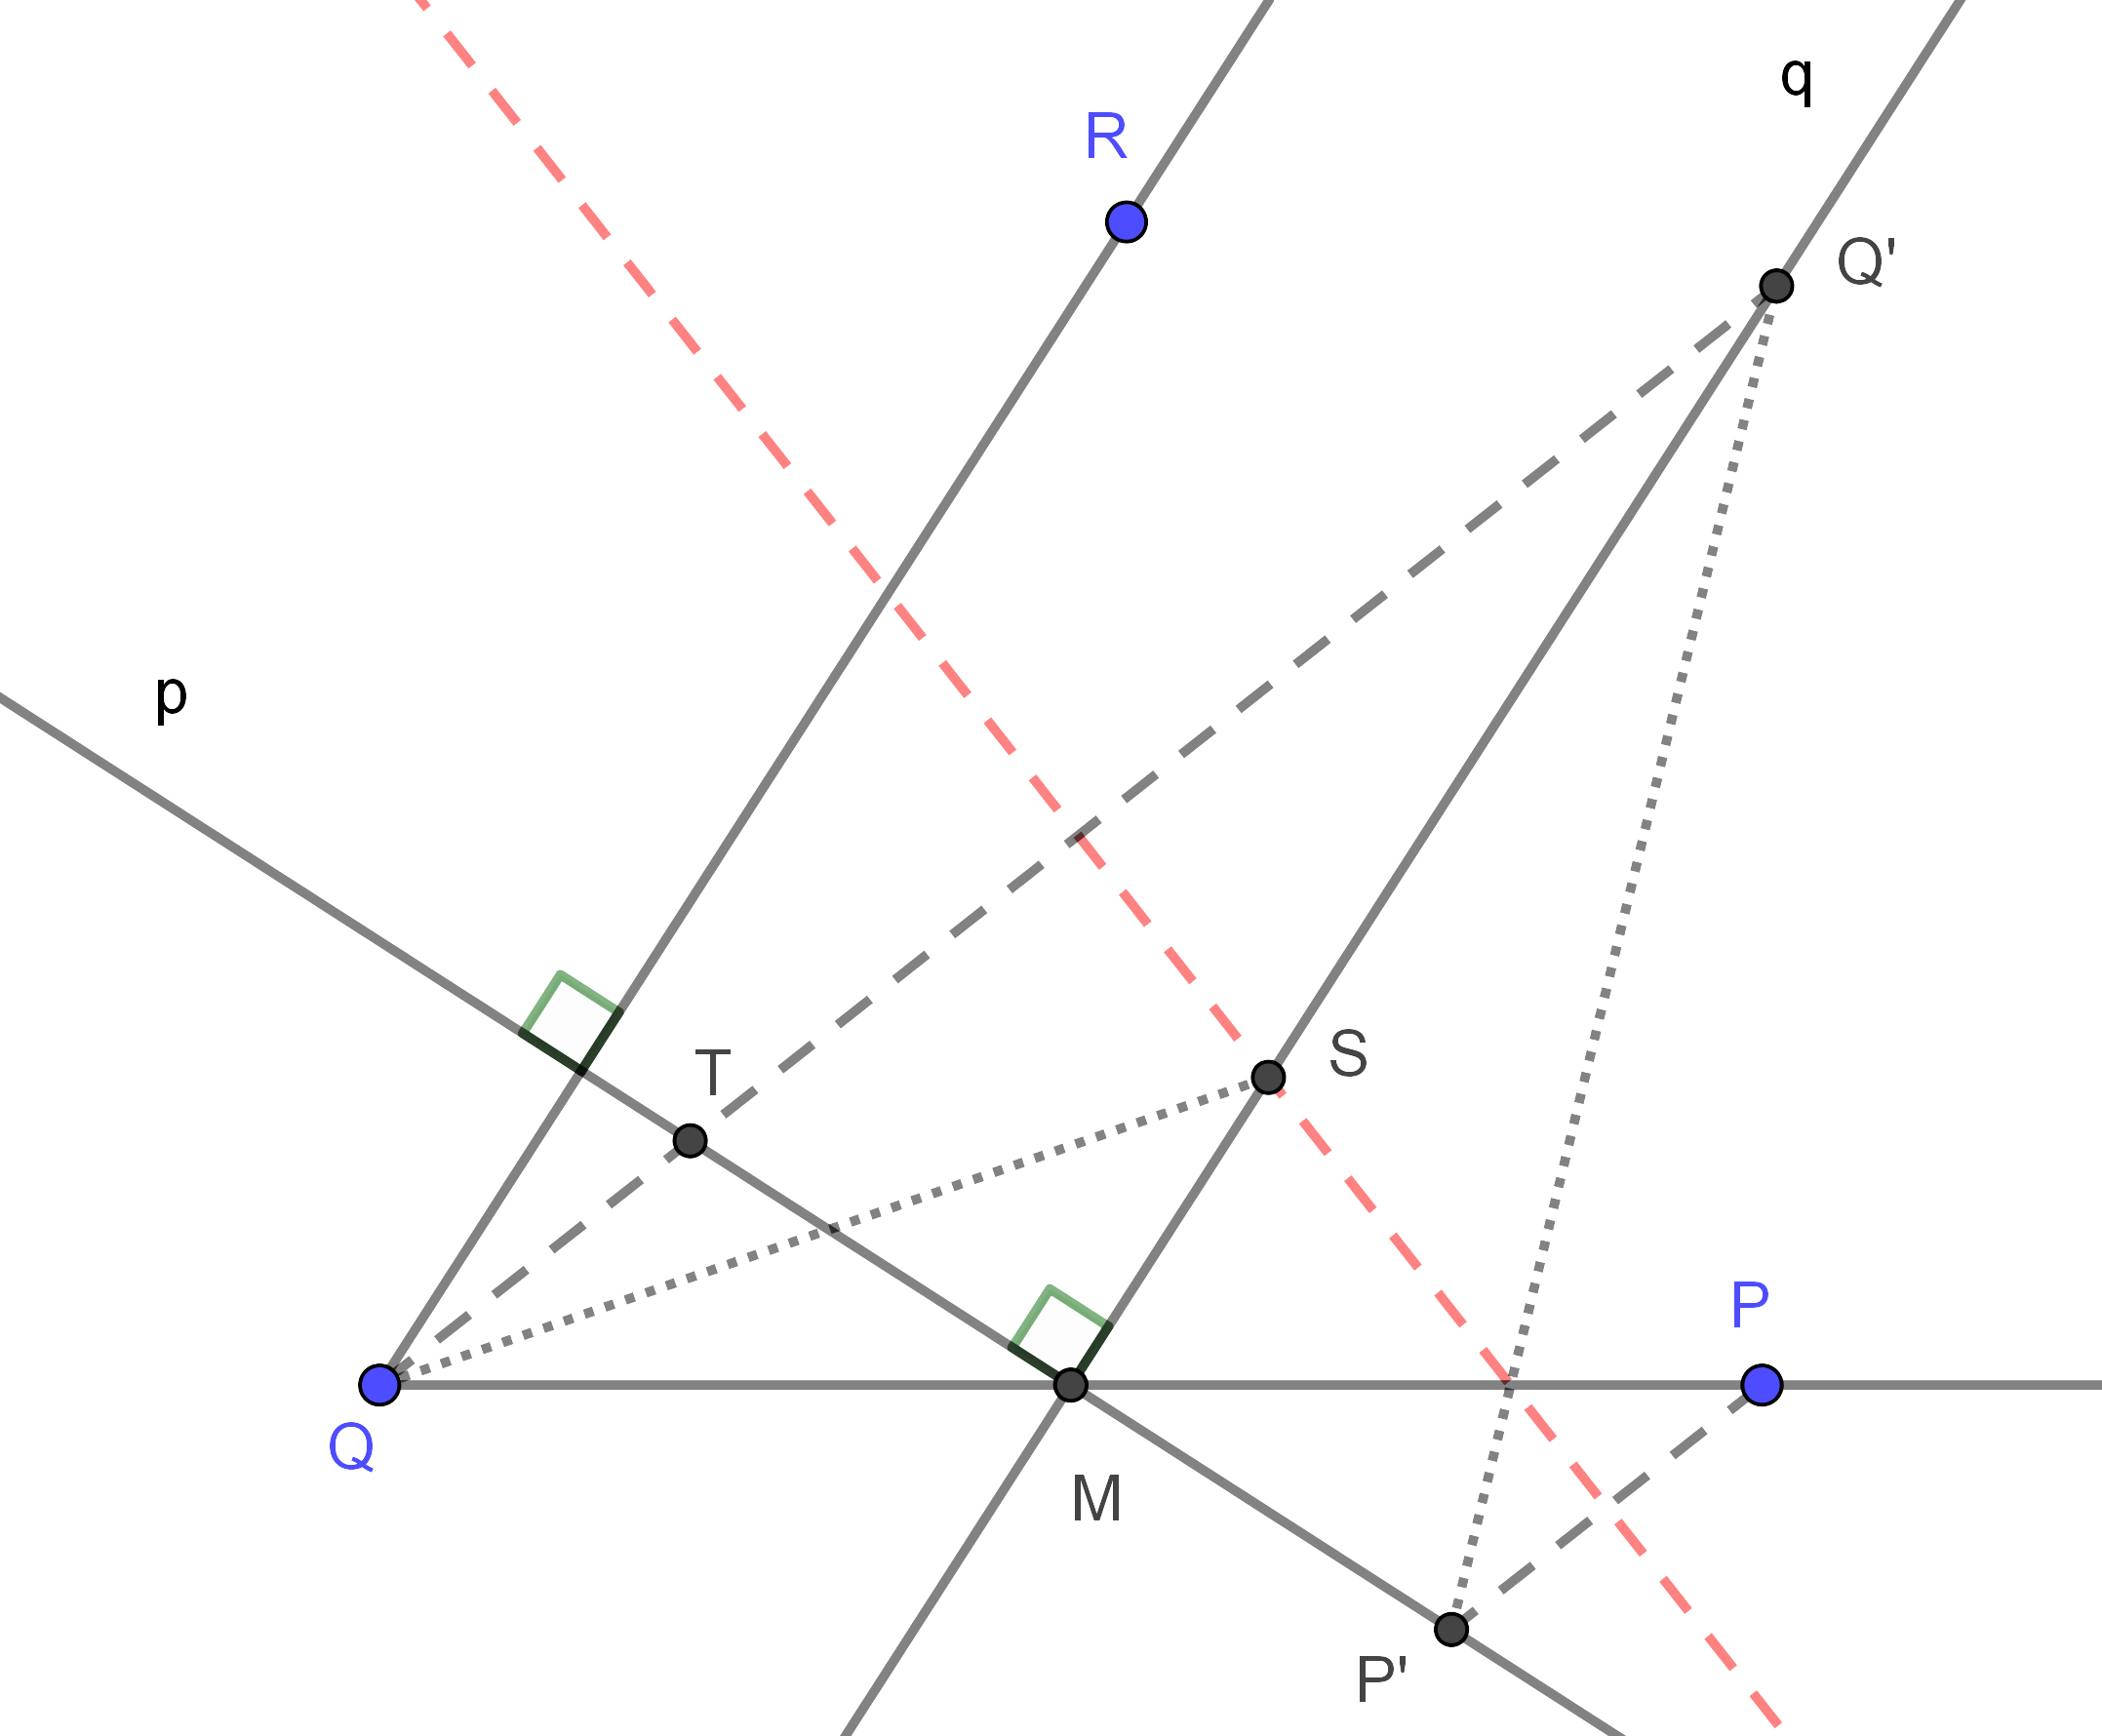
\includegraphics[width=0.5\textwidth]{images/starogr_problemi/trisection_10.4.png}
    \caption[Martinova trisekcija ostrega kota (metoda $1$)]{Martinov postopek za trisekcijo kota iz~\cite[str.\ 154]{geometricconstructions}.}
    \label{fig:trisection_10.4}
\end{figure}

\begin{trditev}
    Daljici $QT$ in $QS$ tretjinita kot $\angle PQR$.
\end{trditev}
\begin{dokaz}
    Ker velja $|QM| = |MP|$, $\angle PMP' = \angle TMQ$ in $QT \parallel PP'$, sta trikotnika $\triangle QMT$ in $\triangle PMP'$ skladna in je $|TM| = |MP'|$. Potem sta skladna tudi pravokotna trikotnika $\triangle TMQ'$ in $\triangle P'MQ'$, zato je $\angle MQ'P' = \angle TQ'M = \angle RQQ'$ (zaradi izmeničnih kotov ob vzporednicah $QR$ in $q$) $= \angle Q'QS$ (ker je trikotnik $\triangle QSQ'$ enakokrak).
    
    Bralec se lahko hitro prepriča, da daljica $Q'P'$ seka pregib ravno v njegovem presečišču z daljico $MP$ (vsi koti ob tem presečišču so zaradi konstrukcija pregiba in sovršnosti skladni). Zato velja še $\angle PQQ' = \angle P'Q'Q$, iz česar sledi
    $$ \angle MQS = \angle SQT = \angle TQR.$$
\end{dokaz}

Druga metoda je prvi zelo podobna. Zopet vzamemo oster kot $\angle PQR$ in s točko $M$ označimo središče daljice $PQ$. Naj bo $l$ pravokotnica na $QR$ skozi točko $Q$, točka $N$ nožišče pravokotnice na premico $l$ skozi točko $P$, s $q$ označimo pa še pravokotnico na premico $l$ skozi točko $M$. Opravimo tisti Belochin pregib, ki točko $Q$ položi na premico $q$ (v točko $Q'$) in točko $N$ na poltrak $QR$. Naj bo točka $S$ presečišče pregiba s premico $q$ (slika~\ref{fig:trisection_10.14}).

\begin{figure}[h]
    \centering
    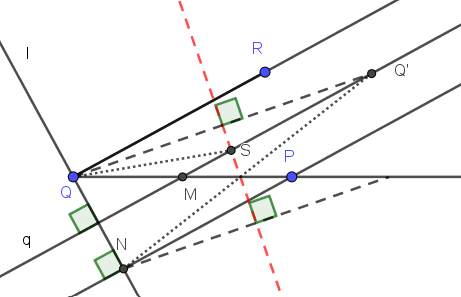
\includegraphics[width=0.6\textwidth]{images/starogr_problemi/trisection_10.14.png}
    \caption[Martinova trisekcija ostrega kota (metoda $2$)]{Martinov postopek za trisekcijo kota iz~\cite[str.\ 158--159]{geometricconstructions}.}
    \label{fig:trisection_10.14}
\end{figure}

\begin{trditev}
    Daljici $QQ'$ in $QS$ tretjinita kot $\angle PQR$.
\end{trditev}
\begin{dokaz}
    Zopet premislimo, da se pregib, poltrak $QP$ in daljica $NQ'$ sekajo v isti točki. Zato je $\angle QQ'N = \angle PQQ'$. Zaradi vzporednosti kraka $QR$ in premice $q$ sta skladna tudi izmenična kota $\angle RQQ'$ in $\angle QQ'S$, z njima pa je zaradi enakokrakosti trikotnika $\triangle QSQ'$ skladen tudi kot $\angle SQQ'$.

    Ker velja $|QM| = |MP|$ in $q \parallel NP$, je premica $q$ simetrala daljice $QN$, torej tudi simetrala kota $\angle QQ'N$. Iz tega sledi
    $$ \angle MQS = \angle SQQ' = \angle Q'QR.$$
\end{dokaz}